\section{WORKBOOK LESSON 3
THE TWELVE ASCENDANTS AND SAMPLE CHARTS}
 

In this lesson we will present a chart for each of the twelve Ascendants. This will help you understand the different rules, dynamics, energetics and relationships between the planets that vary radically by Ascendant. Each Ascendant is a new game, as it were, with different rules of position and aspect.

We have presented the South Indian chart but have done the Bhava or House Chart in the North Indian style, as the North chart is better for reading houses as we indicated in the last lesson.

 

\subsection{Aries Ascendant Chart}
 

\paragraph{Nature of Aries Ascendant}

 

Aries is a headstrong and assertive Ascendant, generally of a Pitta or fiery nature. Friendly planets are Jupiter, Moon, Sun, and Mars. Unfriendly planets are Mercury, Venus and Saturn. There is no single Yoga Karaka planet. This is caused primarily by the combination of the Sun and the Moon as fourth and fifth lords. Jupiter, though generally good, is slightly tainted by its twelfth house rulership. Mars is tainted by its eighth house rulership. Saturn is the worst planet, followed by Mercury and Venus.

 
\begin{figure}[h]
\centering
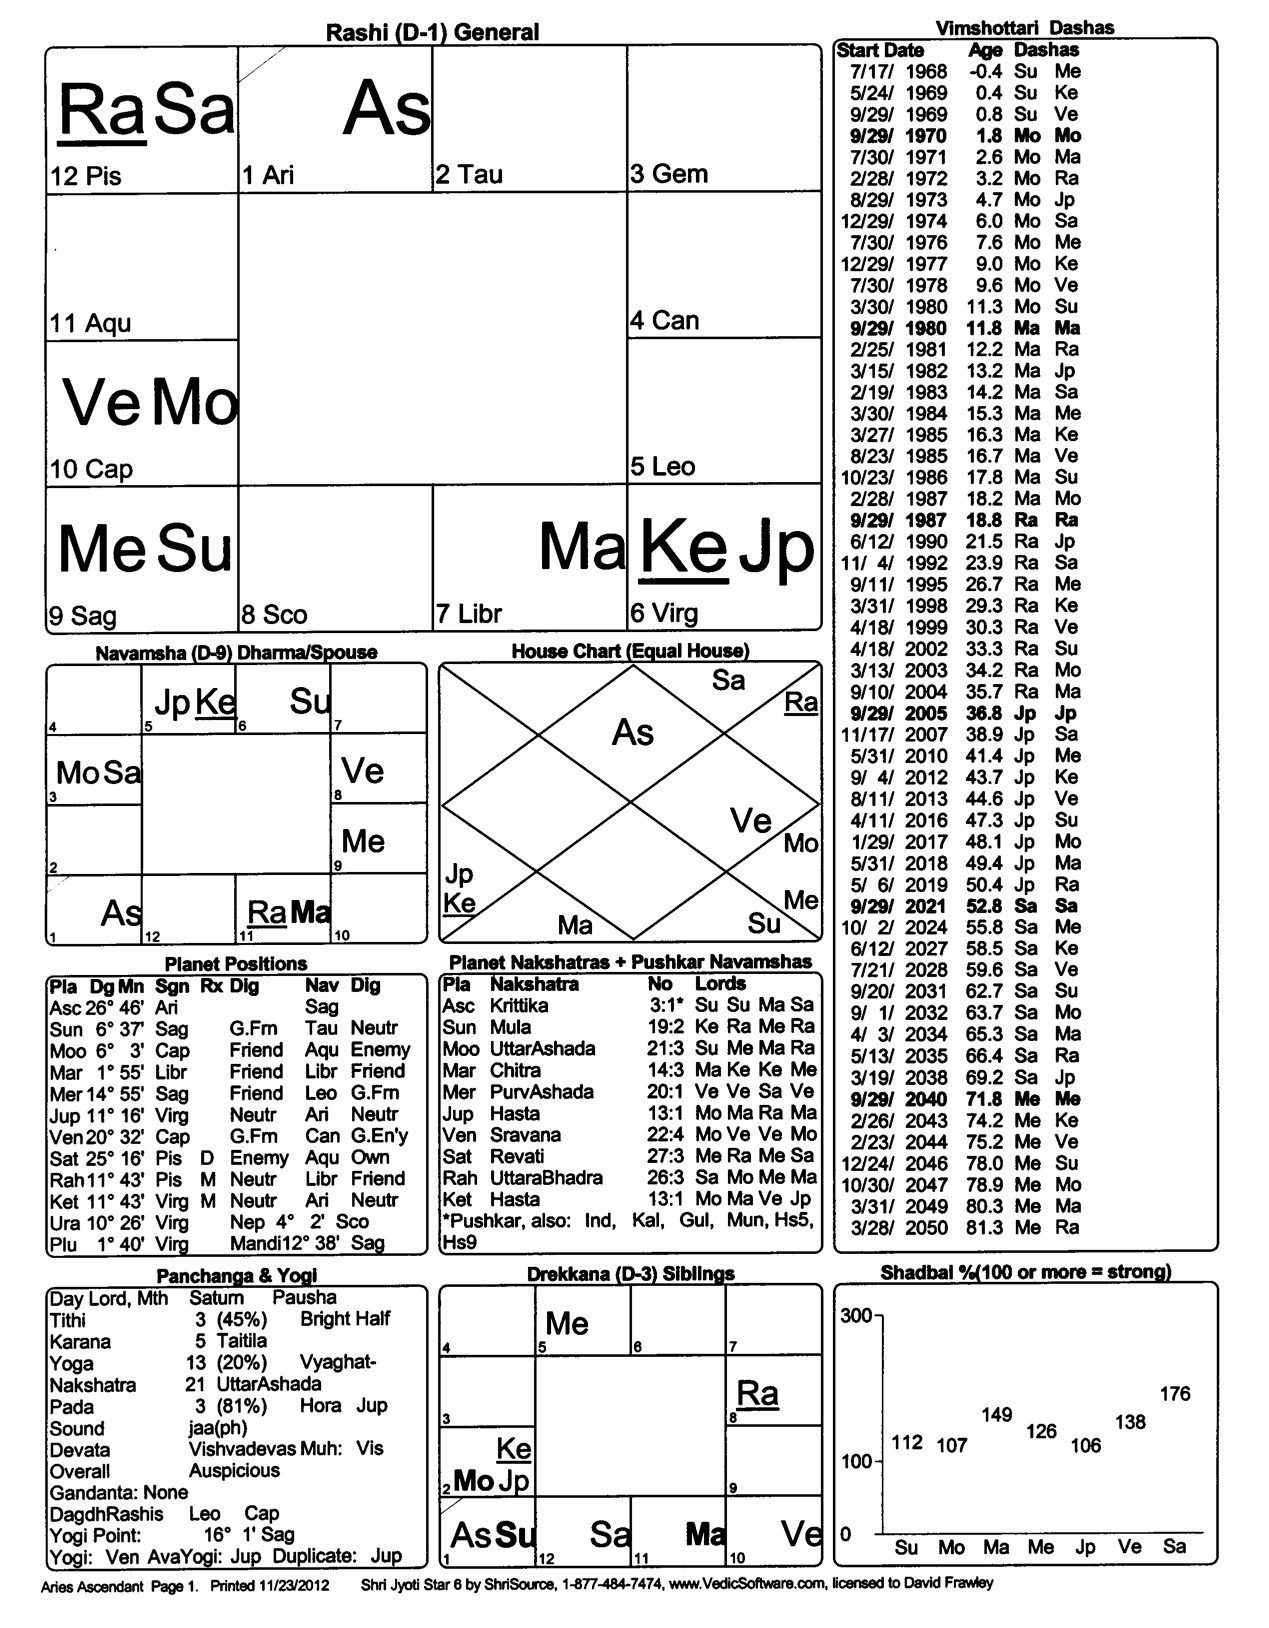
\includegraphics[width=10cm]{pics/Aries-Ascendant.jpg}
\caption{}
\end{figure}


Indications of Sample Chart

 

The chart is of a young doctor and teacher of medicine, recently married and with a child due in March of 1997. He was an adopted child and came from a humble background but has been very successful primarily owing to his own efforts and initiative. He is highly intelligent and sociable, with a strong physique and is a good athlete.

 

First note the position of all the planets as house lords in different houses. The lord of the first, Mars, has gone over into the seventh house. This strengthens the Ascendant because its own lord aspects it. Yet because Mars is also lord of the eighth, the person is a bit daring and reckless. He likes to ride motorcycles and has gotten into a few minor accidents. The position of Mars here does constitute a Kuja Dosha and aspects the seventh lord Venus.

 

Venus, lord of the second and seventh, goes to the tenth. This gives an attractive and extroverted partner, who shares in his work and public life. It is excellent for career and income (second house). The Moon also located here strengthens these possibilities. Moon, lord of the fourth, goes into the tenth. This gives a happy combination of home and career and makes the person popular and good at working with people. It also gives property gains through ones occupation.

 

Mercury, lord of the third and sixth, goes into the ninth house of education. This provides a good education and good learning abilities. Along with the Sun, the fifth lord, or ninth from the ninth, it raises the natives intelligence yet further and makes him a good teacher and writer. Mercury in Sagittarius is in an exchange with Jupiter in Virgo. This is an auspicious combination for teaching and writing about health (sixth house and sixth sign).

 

Sun, lord of the fifth, goes into the ninth. This gives a good mind (buddhi) and good education, high status and also raises the status of the children. The native has a strong sense of Dharma.

 

Jupiter, lord of the ninth and twelfth, goes into the sixth house of health and disease. This makes the person hard working and contributes to him being a doctor. Its aspect to the tenth boosts up the career potential. The mutual aspect with Saturn, the tenth lord, constitutes a Raja Yoga. Curiously the natives work is not only with health (sixth house) but with foreign health systems (Chinese medicine and Ayurveda), the twelfth house.

 

Saturn, lord of the tenth and eleventh, goes into the twelfth house. This gives a degree of renunciation to the persons character and helps enhance spirituality. However it does show shifts and breaks in the career (tenth house) and income (eleventh house), and possible stress and overwork. Dashas and Bhuktis of Saturn should be treated with great caution in regard to these matter. Saturns aspect on the Sun, however, is good for doctors and is found in many doctor charts. It gives seriousness and concentration.

 

The Rahu-Ketu axis falls along the twelfth and sixth houses, which is generally a good place for it, and is helpful for a doctor or healer, giving healing powers and also helping them ward off disease or difficulty. The chart has a weak Kala Sarpa Yoga (all the planets between Rahu and Ketu) because Saturn is located outside of Ketu.

 

Positions from the Moon Sign

 

Relative to the Moon sign the positions are from Capricorn. The Moon is the lord of the seventh from the Moon sign along with Venus. This enhances marriage and partnership and counters some of the afflictions of the seventh house in the sign chart. Venus, lord of the fifth and tenth and Yoga Karaka for Capricorn is with the Moon. This increases income and success in life.

 

Saturn, lord of the first and second houses from the Moon, is well placed in the third house giving work ability and a competitive spirit. The person is also an athlete. Jupiter, lord of the third and twelfth from the Moon, is located in the ninth from the Moon, again enhancing education and sense of Dharma. With Ketu it gains a more spiritual sense.

 

Mars, lord of the fourth and eleventh from the Moon, is located in the tenth from the Moon. This boosts up the career and makes the person ambitious and hardworking. It has further strength because it aspects Venus, the tenth lord.

 

Mercury, lord of the sixth and ninth from the Moon, is located in the twelfth from the Moon. This aids in spiritual growth and a sense of service. Its exchange with Jupiter is now with the ninth and twelfth houses, emphasizing this spiritual quality. The Sun, as the ruler of the eighth from the Moon, is located twelfth from it. This is also a good position for spirituality and selfless service.

 

Separation from the birth father is clearly indicated in the chart. Saturn aspects the Sun in Sagittarius with its tenth aspect. It also aspects the ninth house of the father, and Jupiter, the ruler of the ninth house. Jupiter, the ruler of the ninth house of the father, is on the Rahu-Ketu axis showing something unusual about the relationship. Similarly Saturn aspects the ninth house from the Moon (Virgo) and its lord Mercury, showing the same thing.

 

\subsection{Taurus Ascendant Chart}
 

\paragraph{Nature of Taurus Ascendant}

 

Taurus Ascendant inclines one to earthly and Venusian pursuits. Friendly planets are Mercury, Venus and Saturn. Unfriendly planets are the Sun, Moon, Mars, and Jupiter. Venus is tainted by its rulership of the sixth house. Mercury is slightly tainted by its rulership of the second. The Sun as a malefic benefits by its rulership of the fourth, an angle. Mars is a Maraka. Jupiter is particularly inauspicious.

 
\begin{figure}[h]
\centering
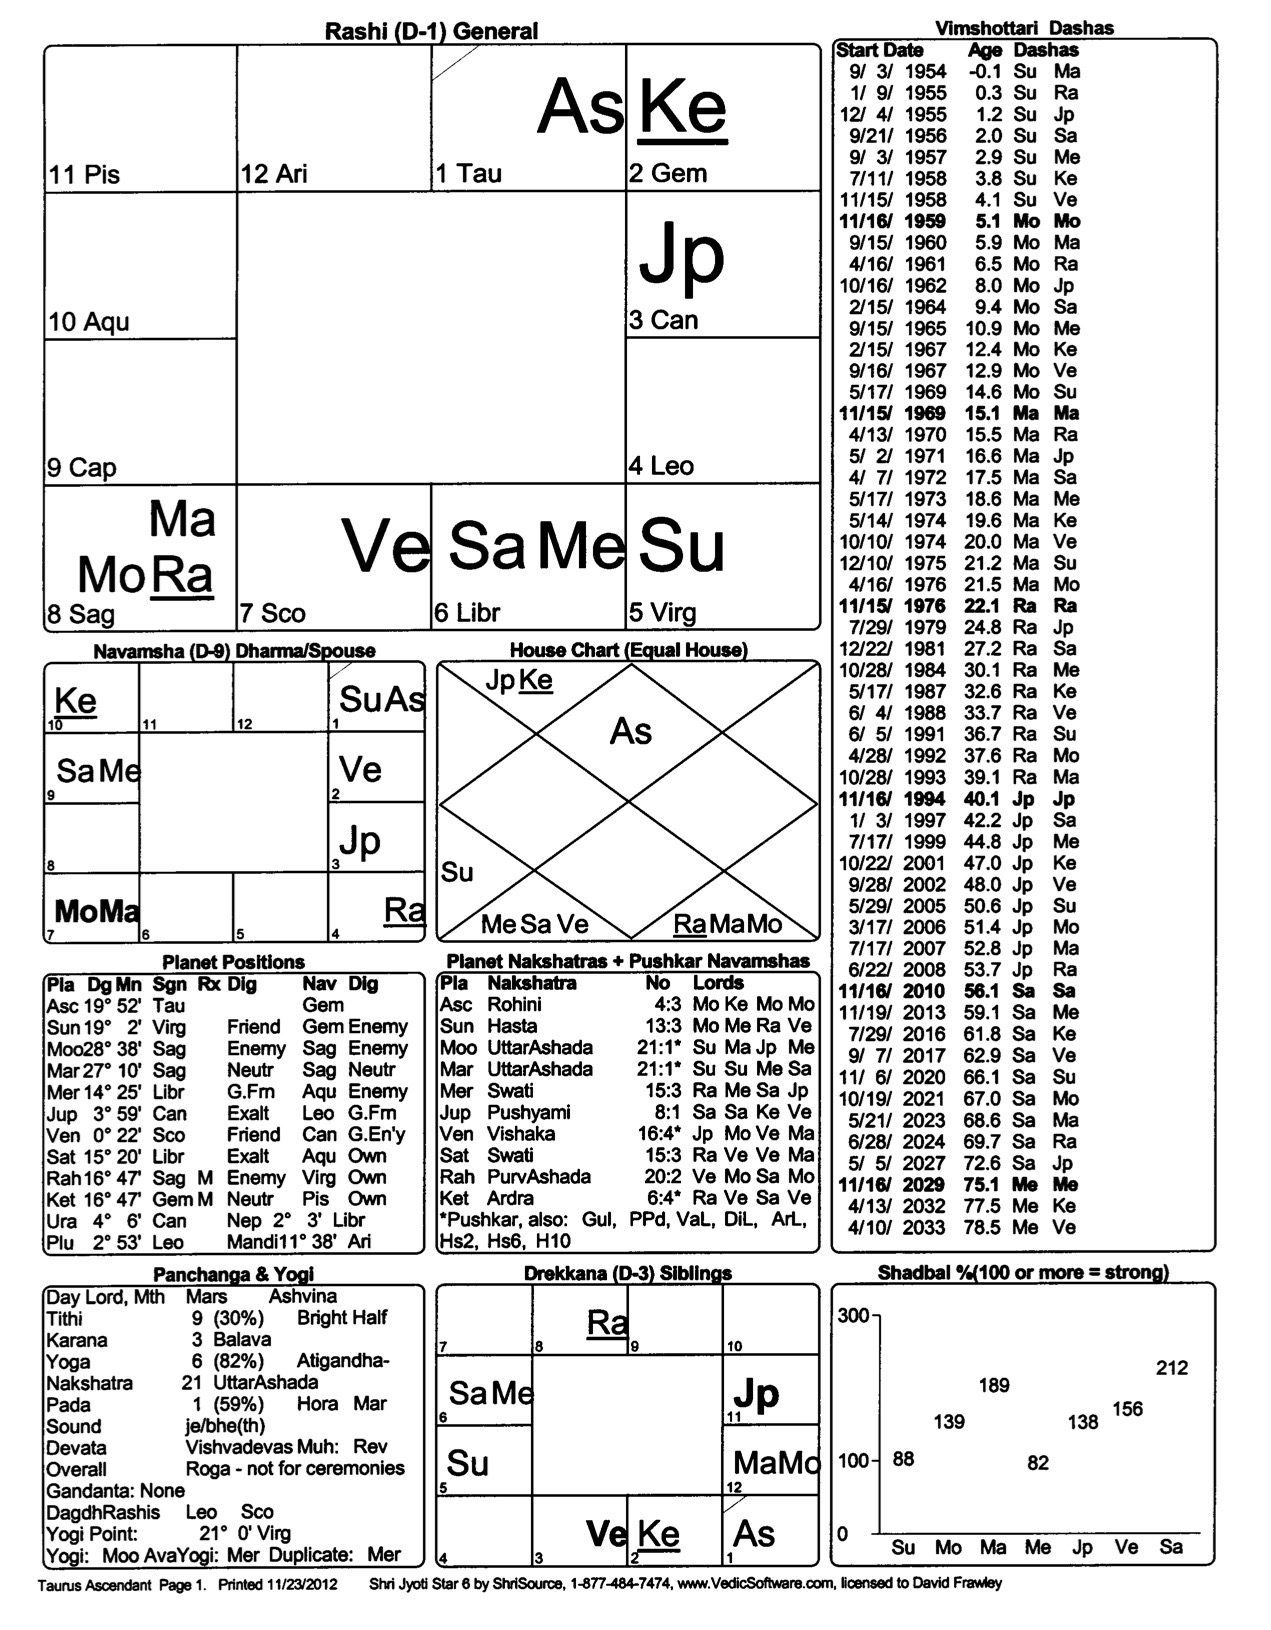
\includegraphics[width=10cm]{pics/Taurus-Ascendant.jpg}
\caption{}
\end{figure}


\paragraph{Indications of Sample Chart}

 

This is the chart of a woman and an artist with considerable talents in painting, sculpture and design, but as yet not a lot of outward success in life. Like many artists her personal and emotional life has been turbulent and erratic. She has had a number of ups and downs in career and relationship and has no children. However she has a strong spiritual inclination that continues to develop.

 

Venus, the lord of the Lagna, goes to the seventh house of relationship. Its aspect on its own sign, the Ascendant, makes the individual attractive and somewhat sensual. While this strengthens the Ascendant, Venus in the seventh house causes complications for relationship.

 

Mercury, lord of the second and fifth, goes into the sixth house of work and disease. The native has a sensitive nervous disposition but also an ability for painstaking crafts work, with many manual skills and much dexterity.

 

The Moon, lord of the third house of brothers and sisters and vital energy, goes into the eighth house, where it is afflicted by Mars, Rahu and Saturn. The conjunction with Mars is to less than a degree. This can make her emotionally unstable and also causes difficulty with her siblings. The third lord (vital passion) in the eighth, a Duhsthana, makes a person emotionally impulsive and sometimes reckless. There is also an exchange between the Moon (Sagittarius) and Jupiter (Cancer) that brings a spiritual potential to this combination. Any combination Mars/Saturn influence on the Moon can turn a person into a loner, a recluse, or an ascetic.

 

The Sun, lord of the fourth house, goes into the fifth house. There it denies children to her, but gives a good creative intelligence and a good education.

 

Jupiter, lord of the eighth and eleventh houses, goes into the third house. There it gives strong artistic abilities (third house relates to art) and the capacity for the fine arts (exalted Jupiter). Jupiter aspects the seventh house boosting up its potential. Yet even though exalted it cannot give her a good marriage. This is not only because of the affliction of the seventh lord, Jupiter as the dispositor of these difficult planets in the eighth house further casts their negative influence on the seventh house.

 

Saturn, lord of the ninth and tenth houses, is exalted in the sixth house. This gives a capacity for public recognition through hard work and effort, and along with Mercury, lord of the fifth, a trine, constitutes a Raja Yoga.

 

The Rahu-Ketu axis runs along houses eight and two, which is a difficult combination. Rahu in the eighth causes many problems in life, including emotional and nervous difficulties. The affliction of the second house causes trouble with finances as well, particularly considering that the second lord is in the difficult sixth house along with Saturn. The chart has a weak Kalasarpa Yoga (all the planets between Rahu and Ketu) but the Moon and Mars extend beyond the position of Rahu.

 
\paragraph{Positions from the Moon Sign}

 

The Moon is clearly highly afflicted in this chart, being located in Sagittarius, from which it is the eighth lord, along with malefic Mars and Rahu and aspected by Saturn. When the Moon is highly afflicted the other good potentials in the chart cannot always manifest. A weak Moon can give either weak health or a unstable emotional nature. In either case a person is inhibited in life, even if avenues of success are available to them. In this particular chart the weak Moon limits other potentials from developing, though it can give the person a spiritual orientation. The person must learn the lesson of renunciation.

 

The Moon is in an exchange with the lord of the Moon sign Jupiter, as first and eighth lords. This is good for spirituality but causes obstructions as a first-eight relationship. Here we see how two benefics and natural friends exchanging signs may not bring good results if the houses are not good. Mars aspects both the Moon and Jupiter, however, causing additional complications.

 

The seventh from the Moon gets afflicted along with the Moon. Saturn also conjoins the lord of the seventh, limiting it further. Mercury and Saturn are in the eleventh from the Moon as rulers of houses four and seven, and two and three. This gives a good income potential. Venus, as the sixth and eleventh ruler, located in the twelfth from the Moon further adds to the artistic disposition. The Sun in the tenth from the Moon as the ninth lord gives possible great career gains.

 

\paragraph{The Navamsha}

 

The Navamsha shows a very strong ninth house, with Saturn, the ninth lord in the ninth along with the Ascendant lord Mercury, affirming a good spiritual potential. The Moon is afflicted by the Sun and Mars in the seventh house, showing additional complications in that area. The Moon and Mars are both vargottama, making them stronger but not necessarily more benefic.

 

\subsection{Gemini Ascendant Chart}
 

\paragraph{Nature of Gemini Ascendant}

 

Gemini is a sign of communication, business, and intellectual pursuits. It is a sign of mixed strength. It is ruled by Mercury, not a strong planet, and has no single Yoga Karaka planet, though some astrologers would see Mercury, lord of the first and fourth, an angle and a trine as being this. Saturn, though a natural friend with Mercury, gives mixed results as the eighth and ninth lord. Venus, though generally good is still blemished by its twelfth house ownership. Mars is the worst planet as lord of the sixth and eleventh. The Moon becomes a maraka but is otherwise rather neutral. The Sun as the third lord is inimical.

 
\begin{figure}[h]
\centering
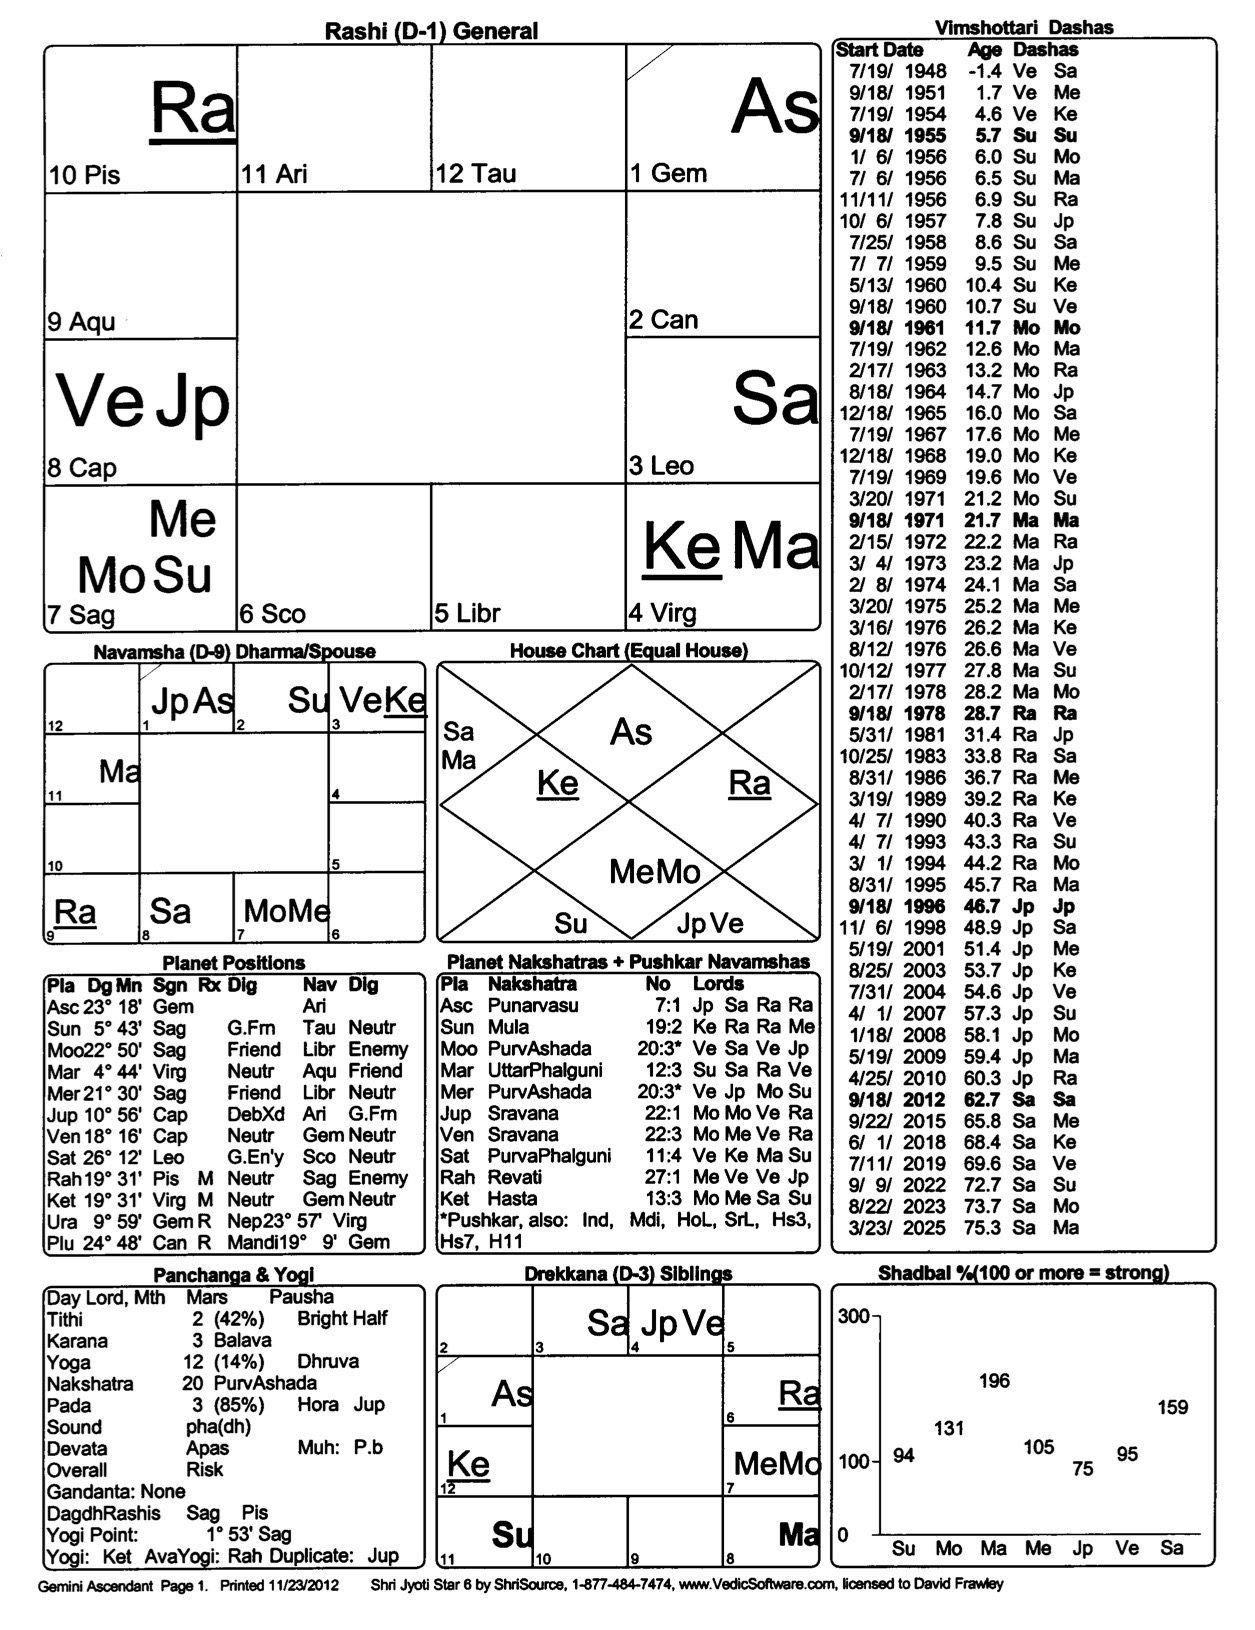
\includegraphics[width=10cm]{pics/Gemini-Ascendant.jpg}
\caption{}
\end{figure}


\paragraph{Indications of Sample Chart}

 

The native is an astrologer and a good speaker and writer. He has done excellent research into astrology (Western) and has a very innovative, profound and detailed mind. However he has suffered from career, health and relationship difficulties, particularly in recent years.

 

Mercury, the lord of the first and fourth houses, goes to the seventh house. This strengthens the Ascendant as it is aspected by its lord, making the person highly communicative and intelligent. However along with the Sun and the Moon it weakens the seventh house making it unstable.

 

The Moon as lord of the second house in an angle increases writing and speaking abilities but imbalances the seventh house. The Moon is in the same sign as the Sun and so fairly weak in brightness. A weak Moon in the seventh causes emotional instability in relationship. The Sun as lord of the third house, also goes into the seventh house, which is not a good placement for it. The Sun in the seventh makes relationship difficult, particularly for a woman, but also for a man, though it can strengthen the career. The third lord here causes impulsiveness in relationship. This further weakens the natives relationship capacity. Not only is the new Moon combination disturbing, the addition of Mercury makes relationship particularly emotionally difficult for the native. On top of this Mars as the malefic sixth and eighth lord casts its aspect on the seventh house.

 

Venus, lord of the fifth and twelfth houses, goes into the eighth house. This denies children and marriage to the native as well. However it boosts the spiritual potential and deepens the intelligence (fifth lord of intelligence in eighth house of profundity), particularly since it is not afflicted. It is a good position for astrology.

 

Mars, lord of the sixth and eleventh houses, and a very harmful planet for Gemini, goes into the fourth house of home and happiness. This denies domestic happiness for the native, which has yet to occur for the person.

 

Jupiter, lord of the seventh and tenth houses of relationship and career, goes into the eighth house of obstruction. This further weakens partnership for the individual and also weakens the health. The career is broken and has many ups and downs, but does involve esoteric or occult subjects (eighth house) like astrology. Clearly with such an afflicted seventh house and seventh lord it would be difficult to recommend marriage for this person. If such a person does get married, the partner would be likely to suffer or die prematurely.

 

Saturn, lord of the eighth and ninth houses, goes to the third house of vital energy. This gives some work stamina for the individual, but causes them not to have any younger siblings.

 

The Rahu-Ketu axis is on the fourth-tenth house angle and afflicted by Mars. While Rahu here is generally good and give career gains, with afflictions by Mars and the tenth lord obstructed in the eighth house, these gains may not always fructify.

 

Note the dominance of the chart by malefics in angles (Mars, Sun, Rahu, Ketu) and the Moon and Mercury by association becoming malefic. Meanwhile benefics (Jupiter, Venus) are in Duhsthanas (the eighth), though not afflicted by malefic aspects. Only Saturn is in a good or Upachaya house. Such a chart is much better for the spiritual life than for outer gains.

 

\paragraph{Positions From the Moon}

 

Any time there is a new Moon or grouping of planets with the Moon, the Moon sign becomes more important. Jupiter, lord of the Moon sign and the fourth from it, is in the second house, which is good for income, speech and self-expression.

 

Saturn, lord of the second and third from the Moon, is in the ninth from it. This causes difficulties with luck and with education. Mars, lord of the fifth and twelfth and Yoga Karaka from the Moon, is in the tenth. This is a good position for it and gives career gains, particularly in Mercurial subjects like writing or counseling. Jupiters aspect boosts it up further. But with Ketu there is some harshness or overly critical nature possible.

 

Venus, lord of the sixth and eleventh, is in the second from the Moon. Along with Jupiter it boosts work and income potentials. Mercury, lord of the seventh and tenth from the Moon, is in the Moon sign, with the Sun, the ninth lord, a Raja Yoga. Its association with the Moon, the eighth lord, weakens this Yoga however.

 

Positions are therefore much stronger from the Moon but as the Moon itself is highly afflicted, it will be difficult for these beneficial energies to manifest. The persons own emotional fluctuations may inhibit him from using the opportunities available from the outside. A weak Moon like a weak Lagna can prevent good Yogas in the chart from manifesting, though these will still have some influence during their Dashas.

 

\subsection{Cancer Ascendant Chart}
 

\paragraph{Nature of Cancer Ascendant}

 

Cancer is an Ascendant that links one to the family, society or public, depending upon its disposition. It has a strong Yoga Karaka with the planet Mars. Jupiter, though generally good, is tainted by its sixth house rulership. The Sun, though generally good, is a maraka, as the second lord. Mercury, Venus and Saturn, particularly Saturn become difficult planets.


\begin{figure}[h]
\centering
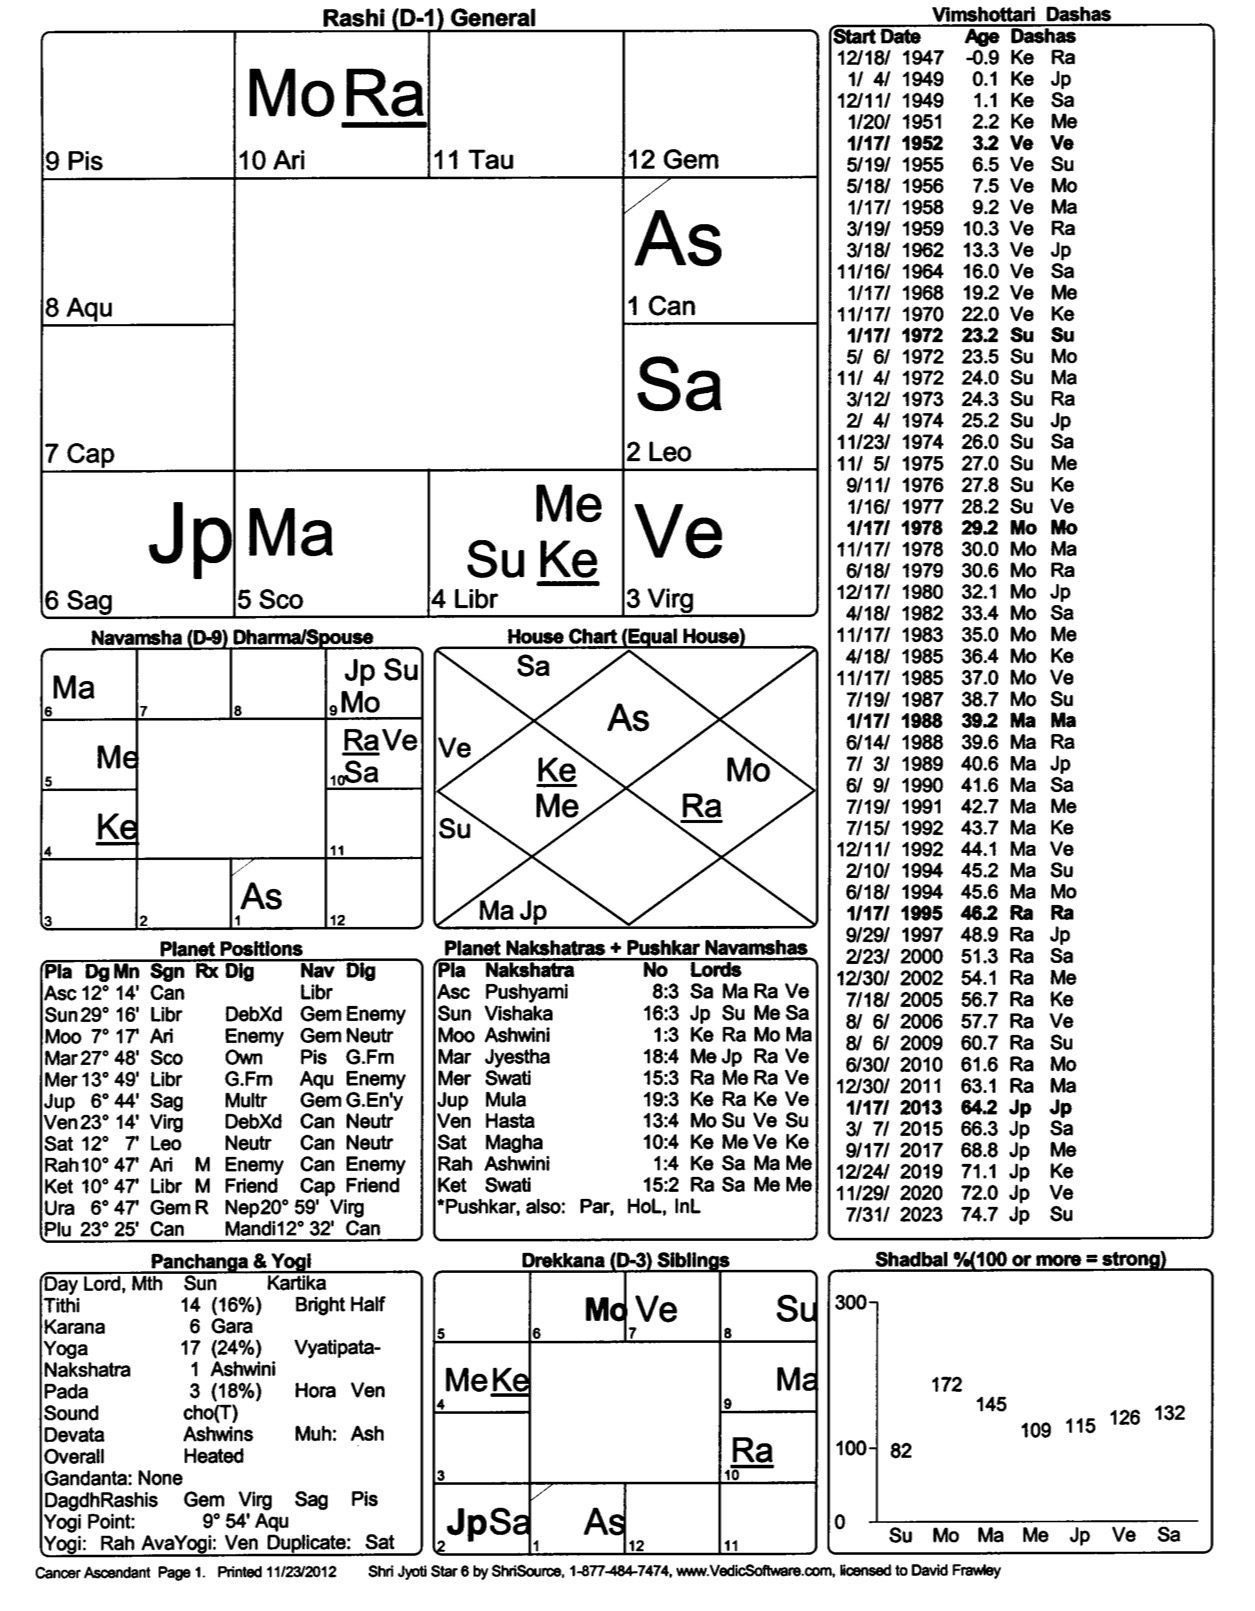
\includegraphics[width=10cm]{pics/Cancer-Ascendant.jpg}
\caption{}
\end{figure}
 

\paragraph{Indications of Sample Chart}

 

This is the chart of Prince Charles of England, whose life is well known and controversial, with his marriage scandal and erratic character. In fact many public and political figures have Cancer Ascendant even if they are not particularly popular or sociable.

 

The Moon, lord of the Lagna, is in the tenth house of career and the public. It is very strong being nearly full, and aspected by benefics like Jupiter and Mercury. However it is afflicted with Rahu, its natural great enemy, with which it is closely conjoined. This gives great fame, power and wealth, and helps make the native a Prince, but touched by scandal and controversy that is bound to be with him as long as he lives.

 

The Sun, lord of the second house of income, is debilitated in the fourth house aspected by the Moon and Saturn, and conjoined with Mercury and Ketu. This gives great properties and strong family ties. However it weakens the character. It also reflects a strong but domineering mother (fourth house) that keeps the native suppressed.

 

Mercury, lord of the third and the twelfth, is also in the fourth house along with the Sun and Ketu. Mercury is opposite the Moon, not considered to be a good aspect for mental peace and stability. This is particularly so because Mercury is in the fourth house of the emotional mind and with Ketu, while the Moon is with Rahu.

 

Venus, lord of the fourth and eleventh houses, is debilitated in the third house. While this has not harmed the native in terms of property and income, his difficulties with women are well-known. Venus and Mercury exchange houses as third and fourth lords, which brings some additional impulsiveness (third house) to the emotions (fourth house).

 

Mars, lord of the fifth and tenth and Yoga Karaka planet, is in its own sign in the fifth house. This is a great source of strength to the native and serves to boost up his children. Mars here gives strength to its other sign, the tenth. Jupiter, lord of the sixth and ninth, is in his own house, the sixth and is unafflicted. This gives the native good health and interest in sports. It helps boost up the tenth house by its aspect.

 

Saturn, lord of the seventh and eighth house, is located in the second house. Note that the ruler of the seventh is located in the eighth house or house of death from the seventh house. As typical of Cancer Ascendant there was both an age and status difference with the wife and an unhappy marriage. Saturn here is not always good for finances for Leo but it has the helping aspect of Jupiter.

 

\paragraph{Positions from the Moon}

 

The Moon is located in Aries as the fourth lord. In mutual full aspect with the Sun, the fifth lord from the Moon, this causes a strong Raja Yoga. The lord of the Moon sign, Mars is located in the eighth house, in its own sign, giving it further strength. The Rahu-Ketu axis along with the Sun and the Moon strengthens this Raja Yoga, but makes it controversial as well.

 

Venus, second and seventh lord from the Moon, is debilitated in the sixth, harming the partner. Mercury, lord of the third and sixth, is in the seventh from the Moon, and as the lord of two difficult houses, further harms the prospects of the seventh house. Mercury and Venus as sixth and seventh lords exchange houses, weakening the seventh house. The debilitated Sun in the seventh, as the fifth lord (romance), harms the seventh house and brings intrigues into it. We see therefore that the seventh house is highly afflicted from the Moon, more so than from the Ascendant.

 

 

Jupiter, the ninth and twelfth lord from the Moon, is in its own sign in the ninth. Aspecting the Moon it boosts up the native in life. Aspecting the fifth it boosts up his progeny. Saturn, the tenth and eleventh lord, is located in the fifth house of children, showing few children and a possible difficult relationship with them. The Rahu-Ketu axis is with the Moon.

 

\paragraph{Navamsha}

 

The Navamsha chart has some significant Raja Yogas as well. Venus, the Lagna lord, and Saturn, the Yoga Karaka, are located in the tenth house giving a Raja Yoga, but again tainted with Rahu. The Moon as the tenth lord is located in the ninth house, another Raja Yoga, along with the Sun, the eleventh lord, giving wealth as well.

 

The Moon is afflicted by the Sun, Jupiter (the sixth lord), and Mars (by aspect) showing emotional turbulence. Mercury in the fifth house of the mind is hemmed in by malefics (Papakartari Yoga). Jupiters aspect to it, as a malefic lord is not entirely helpful. The seventh in the Navamsha is highly afflicted with Saturn aspecting both Venus and the seventh house, and the seventh lord Mars being in the sixth house of enemies.

 

 

The chart is basically quite strong but has an almost fatal flaw, which is Rahu with the Moon opposite the debilitated Sun and Mercury with Ketu. The persons on mind and emotional state is the problem. Otherwise all fortune shines upon him.

 

\subsection{Leo Ascendant Chart}
 

\paragraph{Nature of Leo Ascendant}

 

Leo is a strong Ascendant giving a powerful but often fixed and inflexible personality. Leos are often successful in life but have high expectations. For this reasons extremes of human character can come under Leo.

 

For Leo, the Moon, a natural friend of the Sun, as the lord of the twelfth can cause some harm. Mars is the best planet and Jupiter, though generally good, still is blemished by its rulership of the eighth house. Saturn is the worst planet, as sixth lord, followed by Venus and Mercury, which becomes a Maraka.

 

\begin{figure}[h]
\centering
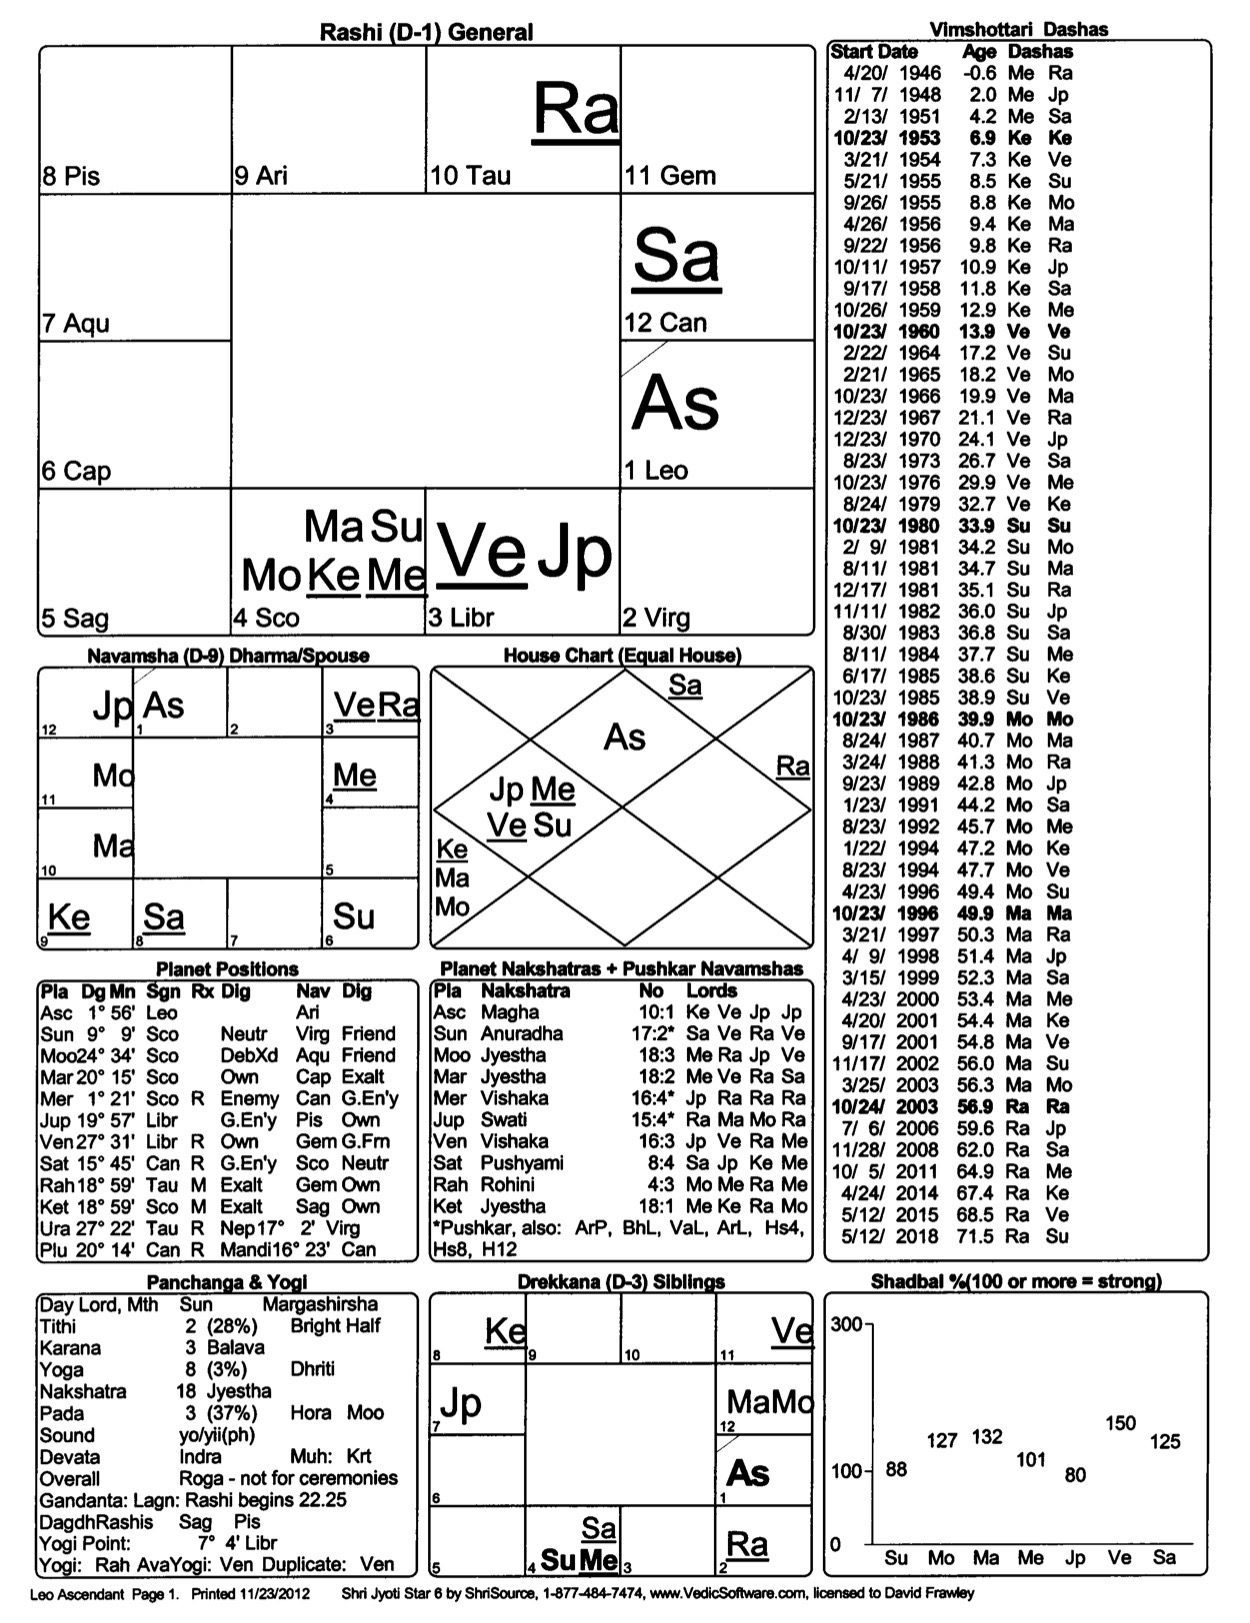
\includegraphics[width=10cm]{pics/Leo-Ascendant.jpg}
\caption{}
\end{figure}
 

 

\paragraph{Indications of Sample Chart}

 

The chart chosen here is from Astrology of the Seers and is of a multiple murderer, Ted Bundy. I thought I would throw in an unusual chart here to make a few points. It is not meant to cast any aspersions against the Leo Ascendant, which, ruled by the Sun, is one of the best and most powerful to have.

 

In this chart nearly all planets are located in the fourth house, which is the house of the heart and emotional nature. The fourth house is highly afflicted with a nearly new Moon (twelfth lord) in debility in Scorpio, the Sun as Ascendant lord, retrograde Mars as Yoga Karaka (fourth and ninth lord), and Ketu. Such a grouping of planets does not create a Sannyasa Yoga (combination of four or more planets in one sign) because it does not include the lord of the tenth.

 

Such combinations of many planets, particularly malefics, are generally inauspicious because the planetary rays get muddled. This is particularly true if they occur in signs ruled by malefics. Both the Moon and Mercury become malefics by association here. A strong Mahapurusha Yoga is created for Mars as the Yoga Karaka for Leo but it is the negative side of Mars that comes out making the person famous as a violent criminal.

 

Jupiter, the fifth lord and eighth lord, along with Venus, the third and tenth lord, are together in the third house, a house of desire (kama). This gives a person energy, curiosity and impulse. It also gives some degree of communicativeness and charisma. Jupiter, as the fifth lord, makes the person clever and adroit at manipulating others, particularly women. Venus suffers by being retrograde as well.

 

Here we see that a combination of Jupiter and Venus, the two most benefic planets, may not be good, particularly when the rest of the chart is so afflicted. It creates sensuality and exaggerated desires. Generally for a criminal to be successful they must have some benefic or good combinations in the chart. Otherwise no one would believe in them. This Jupiter-Venus combination, though hardly simply good, does give the individual enough skill and motivation to succeed in his criminal actions.

 

Bundy was very attractive and charismatic. He generally lured his victims by his personality. He defended himself during his trial and escaped from confinement twice. All of this would not have been possible if he did not have much versatility as well as personal strength.

 

Saturn is retrograde in the twelfth as the sixth and seventh lord. This shows the secretive nature of the native relative to relationship, but it also shows the strong enemies the legal authorities and his time of imprisonment.

 

\paragraph{From the Moon Sign}

 

The Moon sign is Scorpio where the Moon is debilitated. The Moon as ninth lord combines with the tenth lord Sun giving a powerful Raja Yoga but on the dark side. The native was world famous but as a pervert and a criminal. Hence we see that Raja Yogas though they give fame and success may not make a person good. The Moon sign lord Mars is present in his own sign but his sixth lordship, his aggression comes out here. Mercury is retrograde and ruler of two bad houses, eight and eleven, contributing to the deceptiveness and cunning of the person. Ketu keeps this combinations secretive.

 

Jupiter and Venus are in the twelfth from the Moon as second and fifth, and seventh and twelfth lords respectively. This creates secret desires and grandiose wishes. Saturn, as third and fourth lords, is located retrograde in the ninth house, in an inimical sign Cancer. This causes emotional conflict along with perverted values and principles.

 

\paragraph{Navamsha}

 

The Mahapurusha Yoga of Mars exists in this chart as well with an exalted Mars in the tenth house in Capricorn as the Lagna lord. Mars is aspected by cruel Saturn as well from the difficult eighth house. In fact Saturn and Mars exchange signs as the eighth and tenth ruler, linking death and fame. The Moon is also in a sign of Saturn. Venus is with malefic Rahu. Mercury is under the aspect of mars. So the same basic type of negative energies are indicated in this chart as well.

 

\paragraph{Additional Notes}

 

In this chart there are three retrograde planets, while all the other planets but Jupiter are in the Rahu-Ketu axis, which by the retrograde nature of the nodes, always has a retrograde or retarding effect. This contributes to the secretive, deceptive and cruel nature of the person. An emotional nature so saturated with violence shows a Rakshasa, a demonic entity, in the guise of a human being.

\subsection{Virgo Ascendant Chart}
 

\paragraph{Nature of Virgo Ascendant}

 

Virgo is a difficult Ascendant because from it there are not a lot of benefic house lords. There is no single Yoga Karaka planet (planet that rules both a trine and angular house). From it Jupiter becomes malefic ruling two angles. Meanwhile Saturn, ruling the sixth with its best or mulatrikona house, though a natural friend of Mercury and ruler of the fifth, at best gives mixed results. Mars is quite inimical as third and eighth lord. Venus, though generally good, is also a Maraka by ruling the second house.

 

\begin{figure}[h]
\centering
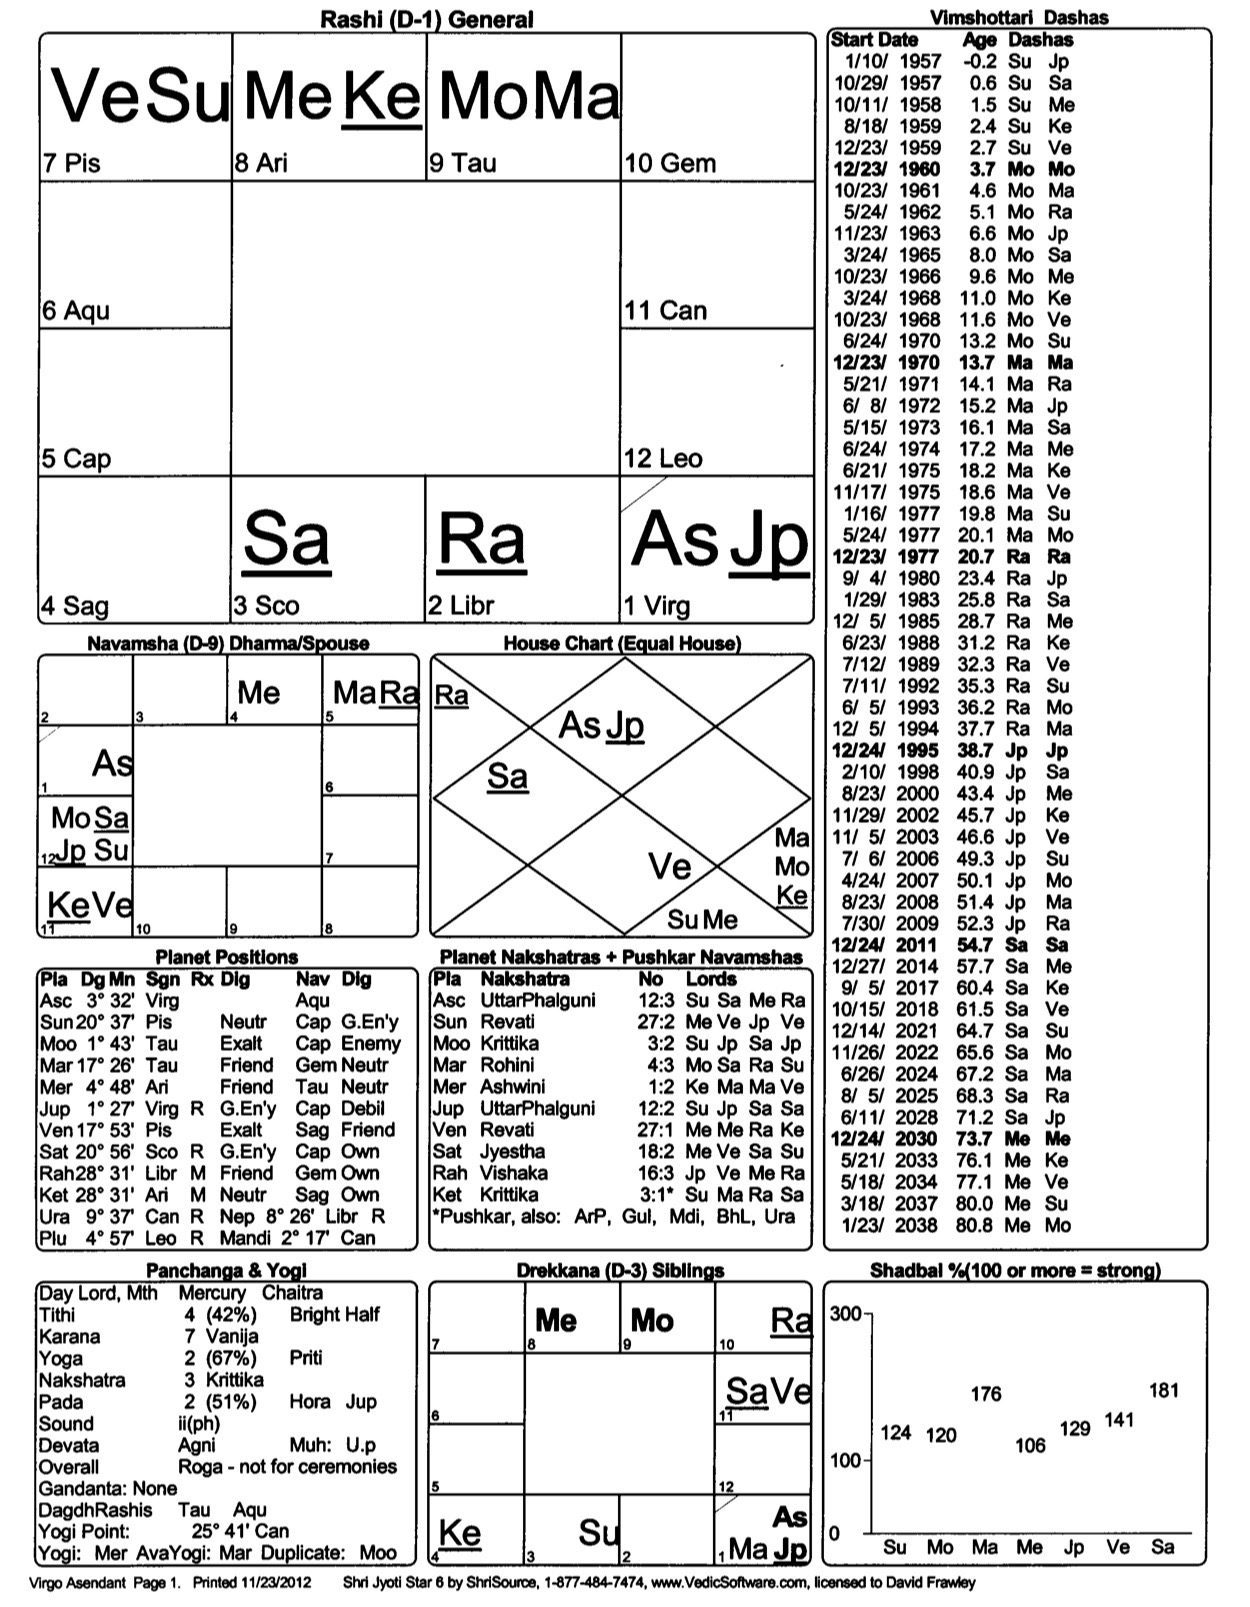
\includegraphics[width=10cm]{pics/Virgo-Ascendant.jpg}
\caption{}
\end{figure}
 

 

\paragraph{Indications of Sample Chart}

 

The individual in this chart is a yoga teacher and massage therapist, who is also a good artist. She has strong spiritual inclinations but both career and relationship difficulties, also living and working in a foreign country. Her health tends to be weak but without major health problems.

 

Mercury, lord of the first and tenth, is located in the malefic eighth house along with Ketu, which is additionally strong being direct in motion. Since this combination is not afflicted it is good for occult and spiritual matters, including Mantra Yoga. However it does weaken the health of the native. In addition the career (tenth lord) is obstructed.

 

Venus, lord of the second and ninth, is well placed exalted in the seventh house. This makes the native, a woman, attractive, communicative and spiritual, creating a Malavya Yoga or Mahapurusha Yoga for Venus. However Venus in the seventh house causes some marital unhappiness, which is compounded by the Sun being there along with it.

 

Mars, lord of the difficult third and eighth houses, and a very difficult planet for Virgo, is placed in the ninth house, along with the Moon. This harms the persons fortune and gives some bad luck and bad timing in life. Yet it also causes them to be open to other religions than that of her birth.

 

Jupiter, lord of the fourth and seventh houses, is located retrograde in the Ascendant. Normally one would think of Jupiter in the Ascendant as good but this is not usually the case for Virgo, owing to Jupiters negative house rulership for it. Jupiter is weakened by being retrograde as well. It gives the person some vitality and self-expression but does not give the good results one might think.

 

As the seventh lord aspecting the seventh house Jupiter does not have the strength to make that house strong, particularly as it is already afflicted. The native has never married. As the natural significator for children aspecting the fifth house, it does not have the power to give her children. As a great natural benefic in the Ascendant, it does not have the power to give her good health. This is a good example of how we must reconsider the role of natural benefics when they become temporal malefics.

 

Saturn, lord of the fifth and sixth houses, is retrograde in the third house. As a malefic in an upachaya house it gives some vital energy and physical stamina, giving an interest in Hatha Yoga. However the aspect of Saturn on the Moon, along with Mars being in the same sign as the Moon, greatly weakens the natives capacity for domestic and emotional happiness (the Moon).

 

The Moon as lord of the eleventh is in the ninth house. The native has received special help and grace through life. However the strong afflictions of the Moon, have prevented this position from giving great gains.

 

The Sun as twelfth lord is located in the seventh house. This is not favorable for marriage but it is favorable for spirituality and for working with foreign countries. The Rahu Ketu axis is between the second and eighth houses. This gives financial limitations and fluctuations.

 

\paragraph{Positions from the Moon}

 

The Moon is exalted in Taurus as the third lord, giving emotional and vital energy to the person. However it is afflicted by Mars, the seventh and twelfth lord, and Saturn, the ninth and tenth lord. This both weakens and spiritualizes the Moon. Saturn is strong in the seventh but afflicting the Moon gives some career gains but little help in terms of domestic happiness.

 

Venus, lord of the Moon, is exalted in the eleventh from it, conjoined with the Sun, the fourth lord, and aspected by Jupiter, the eleventh lord. This gives income potential through Venusian matters, like artistic ventures that can provide a good income for the native.

 

Note that two natural and temporal malefics, Mars and Saturn afflict the seventh from the Moon. The fifth from the Moon is weak with a retrograde Jupiter as eighth and eleventh lord. The second and fifth lord Mercury is weak in the twelfth house, giving some financial obstructions and losses. But it is again good for spirituality, with Ketu in a Moksha house.

 

\paragraph{Navamsha}

 

Four planets dominate the Navamsha, including the Sun, Moon and Lagna lord, in the twelfth house. Saturn in the twelfth is the final dispositor of all the planets in the chart. This twelfth house orientation increases the spiritual disposition of the native and causes her to seek Moksha. It also shows her destiny as connected with foreign countries.

 

The Venus/Mars mutual aspect constitutes a Raja Yoga but this remains weak owing to the strong twelfth house orientation of the chart.

 

\subsection{Libra Ascendant Chart}
 

\paragraph{Nature of Libra Ascendant}

 

Libra is a strong Ascendant being cardinal (movable) and having many possible Raja Yoga combinations. Saturn is the natural Yoga Karaka. The Moon as tenth lord, Mercury as ninth lord, and Venus as lord of the first can also contribute to Raja Yogas. Bad planets are the Sun, Moon, Mars and Jupiter. Yet the Moon as tenth lord can contribute to Raja Yogas. By some accounts even Jupiter can contribute to these.

 

\begin{figure}[h]
\centering
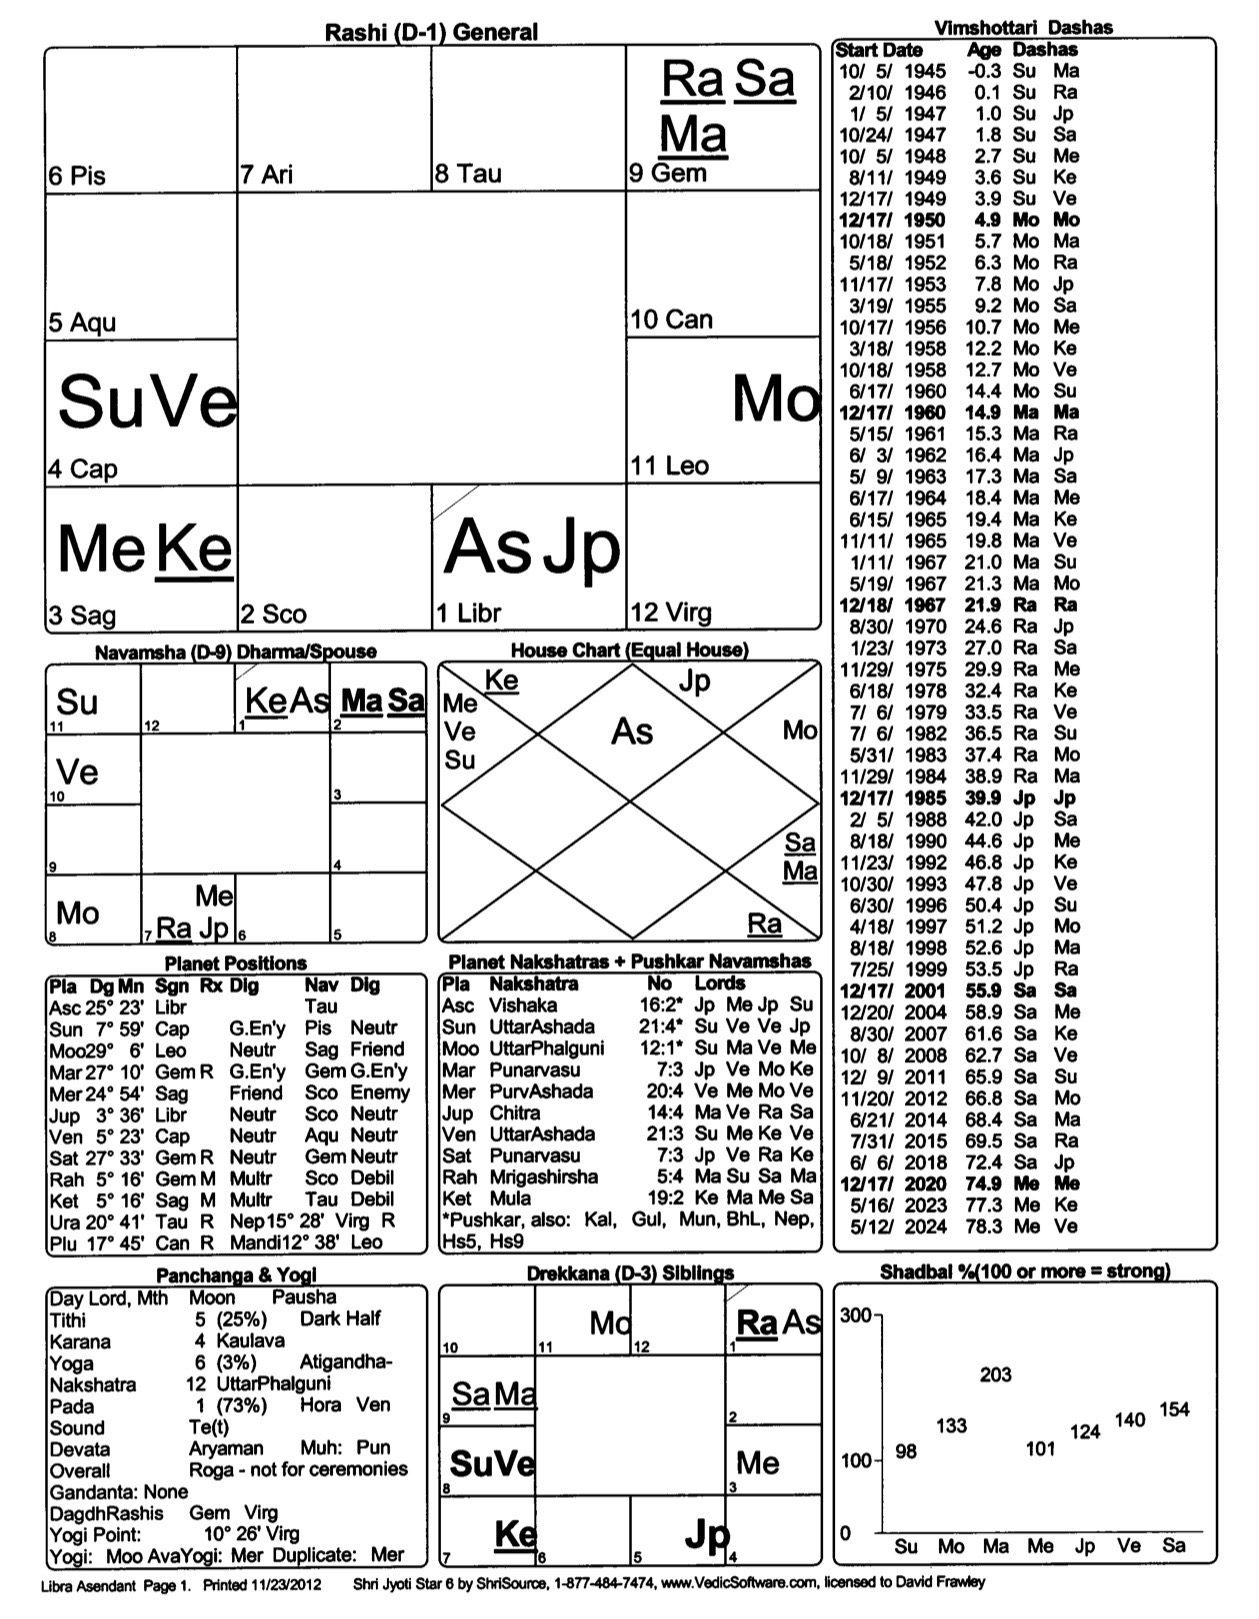
\includegraphics[width=10cm]{pics/Libra-Ascendant.jpg}
\caption{}
\end{figure}
 

 

\paragraph{Indications of Sample Chart}

 

The individual here is a healer, a doctor of natural medicine, an artist and political activist with spiritual and monastic tendencies.

 

Venus, the first and eighth lord, is located in the fourth house along with the Sun, eleventh lord and aspected by Mars. Venus here in an earthly sign and a house of the mind is good for artistic and manual abilities. The Sun, as the eleventh lord, in the fourth house gives gain through property and houses. The native owns a large house that she gained by a special windfall.

 

Mars, the ruler of the second and seventh house, and a maraka planet is located in the ninth house along with malefic Saturn and Rahu. It also aspects Mercury, the lord of the ninth house, and the Sun, the natural karaka for the father. The native lost her father to a heart attack at the age of sixteen, which was during the Mars Dasha, Rahu Bhukti. This position, however, is good for income, with the second and fifth lords in the ninth.

 

Saturn, lord of the fourth and fifth and the Yoga Karaka, is located in the ninth house. Apart from the affliction to the father, this does give it some strength, with a Yoga Karaka in the ninth house. The aspect of Saturn with Mercury, the ninth lord, is a weak Raja Yoga. Mars as the seventh lord, an angular house, does not entirely weaken the Yoga, but as the second lord, does not make it particularly strong. Jupiter adds its aspect to this ninth house combination, giving it more strength.

 

Mercury, the ninth and twelfth lord, is in the third house, where it is afflicted by Ketu, and two retrograde malefics, Mars and Saturn. This can disturb the intellect and judgment of the person but can make them highly philosophical. The native once tried to commit suicide during Rahu-Rahu and almost succeeded. Yet overall she has a highly philosophical, though independent mind.

Jupiter, lord of the third and sixth, two difficult houses, is located in the Ascendant. This makes the native idealistic, self-willed and creative. Though it aspects the seventh house, Aries, and seventh lord, Mars, it does not give an entirely happy married life, though a long marriage did occur under Rahu Dasha.

 

The Moon, the tenth lord, is located in the eleventh house, aspected by Saturn. This gives some emotional pride and strength in Leo along with detachment and aloofness through the influence of Saturn. Gains through profession are indicated as well.

 

The Rahu-Ketu axis falls along the ninth and third houses where it influences the main factors of the mind, Mercury, the second lord and the fifth lord. The individual is creative and philosophical but unorthodox and a rebel.

 

\paragraph{Positions from the Moon}

 

The Moon sign is Leo, from which the Moon is the twelfth lord and aspected by malefic Saturn, the sixth and seventh lord from the Moon. This gives a degree of detachment, renunciation and spirituality to the person, who has a strong monastic bent. The Sun, the lord of the Moon, is in the sixth house from it, where it has some strength as a malefic in an upachaya house. Venus, the third and tenth lord from the Moon, is in the sixth from it and has some weakness, particularly as Mars aspects it.

 

Mars, the fourth and ninth lord from the Moon, is located in the eleventh, with Saturn, the sixth and seventh lord. Such malefics in an upachaya house give gains, particularly relative to Mercurial ventures.

 

Mercury, the second the eleventh lord from the Moon, is located in the fifth house from it and so strongly indicating the mind. Such Mars and Saturn aspects on Mercury, like those on the Moon, can either be deranging or spiritualizing because they deny ordinary fulfillment

 

Jupiter is in the third from the Moon where it aspects the seventh house from the Moon and the seventh lord (Saturn). This gives a spiritualizing effect upon relationship, particularly as Jupiter aspects the same factors (Mars) and the seventh house (Aries) in the birthchart.

 

\paragraph{Navamsha}

 

The Rahu-Ketu axis in the first-seventh axis of the Navamsha causes confusion in relationship. Some astrologers think that it is more difficult in the Navamsha than in the birthchart. Here the position is mitigated by Jupiter and Mercury in the seventh house, though neither are benefic lords for the Ascendant and so are not as good a combination as might appear.

 

From the birthchart one would think that the native might have children, with Jupiter aspecting both the fifth and its lord. However the fifth from the Moon is highly afflicted by Mars and Saturn. In addition the fifth in the Navamsha is highly afflicted by Mars and the Sun. The native has had no children.

 

\subsection{Scorpio Ascendant Chart}
 

\paragraph{Nature of Scorpio Ascendant}

 

Scorpio is an Ascendant of medium strength. It is ruled by a natural malefic Mars, which is tainted by its sixth house rulership. There is no single Yoga Karaka planet but the Sun-Moon combination becomes very strong as the ninth and tenth rulers. Jupiter is generally quite good as second and fifth lord but is still a maraka. Saturn is the worst planet followed by Mercury and Venus.

 
\begin{figure}[h]
\centering
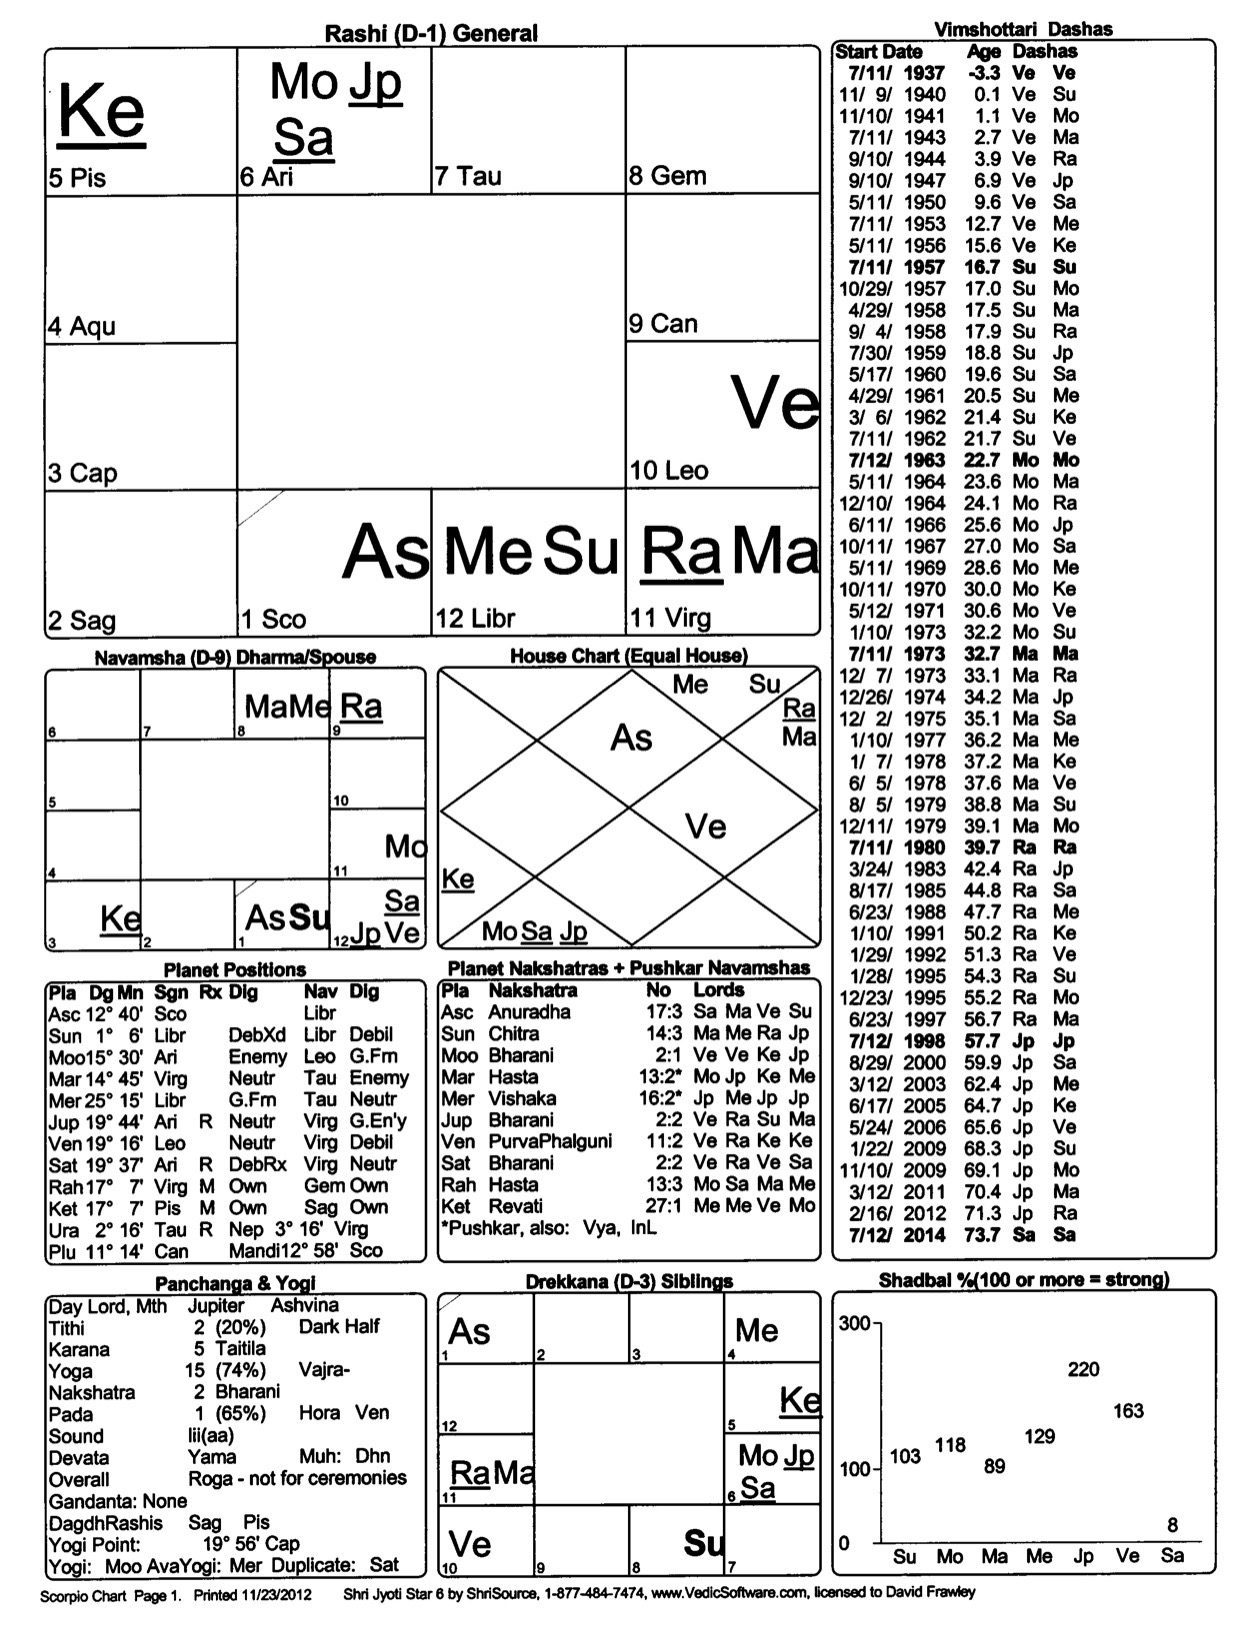
\includegraphics[width=10cm]{pics/Scorpio-Ascendant.jpg}
\caption{}
\end{figure}
 


\paragraph{Indications of Sample Chart}

 

The woman is a successful psychologist, who has gained much recognition for her work, particularly in treating trauma and sexual abuse victims. She is highly spiritual and does much sadhana and meditation. She was married and has a son and a daughter but is now divorced.

 

Mars, the lord of the first and sixth houses, is in the eleventh, an upachaya house, along with Rahu. This gives a good intelligence and counseling abilities, but its affliction to the second house and its lord causes trouble in early childhood.

 

However, what most marks this chart is the grouping of planets along the six/twelve axis. Jupiter, lord of the second and fifth houses, is in the sixth house retrograde. Saturn, lord of the third and fourth houses, is also in the sixth house retrograde. The Moon, lord of the ninth house, is in the sixth house.

 

The Moon is highly afflicted in the sixth house along with retrograde Saturn. Jupiter gives it some benefit but is weakened by its retrograde motion. Mars aspects the Moon, weakening it further. The debilitated Sun as tenth lord and Mercury, lord of the mind, aspect the Moon as well causing more problems. This shows many traumas particularly in the early life, mainly from the Father (Moon as ninth lord, Sun as significator for the father debilitated). The combined influences of Mars and Saturn on the Moon create a Sannyasa Yoga or combination for renunciation. While this greatly limits domestic happiness it can give the ability to transmute ones difficulties in life to a higher plane.

 

More over we must not forget the sixth house as an upachaya house. It gives benefit later on life after obstacles are overcome. The native transmuted her own experience into her career as a psychologist. These sixth house combinations, though causing many afflictions, conceal two important Raja Yogas. Jupiter and Saturn are the fourth and fifth house rulers. The Sun and Moon are in mutual aspect as the ninth and tenth house rulers. This gave the person strength through these afflictions.

 

Mercury, lord of the eighth and eleventh houses, is in the twelfth house. Aspected by the Moon, Saturn and the Sun, the mind is highly sensitive and also reflects a degree of trauma in life, but which has led her toward seeking liberation. The Moon, Mercury, the second, fourth and fifth lords, all the factors of the mind are involved in this combination.

 

Venus, lord of the seventh and twelfth houses, is located in the tenth house, where aspected by Jupiter, it gives career gains. The Sun, lord of the tenth houses, is in the twelfth house. These two exchange their houses. While the placement of the tenth lord in the twelfth generally weaken it, it can also indicate a job in foreign lands, or here involving hospitals or the unconscious (a psychologist).

 

\paragraph{Positions from the Moon}

 

In this chart note that positions are stronger from the Moon. The Jupiter-Saturn combination in the Moon sign is a Raja Yoga combination (as Jupiter rules the ninth and Saturn the tenth from the Moon). The Sun-Moon mutual aspect is another Raja Yoga, the fourth and fifth house rulers. These positions are stronger because they are in an angle to the Moon. Yet the afflictions to the Moon by Mars, Saturn and a debilitated Sun still have their effect. The seventh house from the Moon is most weakened by these influences.

 

Mars, the lord of the Moon sign, along with Rahu, is in the sixth house from the Moon, where malefics usually do well. This gives her stamina and endurance. The Venus-Sun exchange is of the fifth and seventh houses from the Moon. This creates a romantic but impulsive trend to the mind. Ketu as twelfth from the Moon increases the desire for liberation.

 

\paragraph{Additional Notes}

 

This chart shows how a persons experiences in life can be overcome and transmuted into a tool for helping others. At first glance this is a very weak chart, with a highly afflicted Moon in the sixth house. However the Moon is full and Mars, the Lagna lord, is in the eleventh, an upachaya house. In fact most of the planets are in two upachaya houses, the sixth and the eleventh. Hence the native has been able to overcome her difficulties and turn them into strengths. Given the number of retrograde planets in the chart and the Lagna lord with Rahu it appears that this person has been clearing up a lot of past life karma.

 

\subsection{Sagittarius Ascendant Chart}
 

\paragraph{Nature of Sagittarius Ascendant}

 

Sagittarius is a fairly strong Ascendant being the positive sign of Jupiter. However it is not as strong as one might think. There is no single Yoga Karaka planet. The Moon, as lord of the eighth, gains some negative qualities, though it is a natural friend of Jupiter. Natural benefics like Venus and Mercury become inimical. In this regard Sagittarius resembles its opposite sign Gemini, but is stronger because of the greater power of Jupiter over Mercury.

 

\begin{figure}[h]
\centering
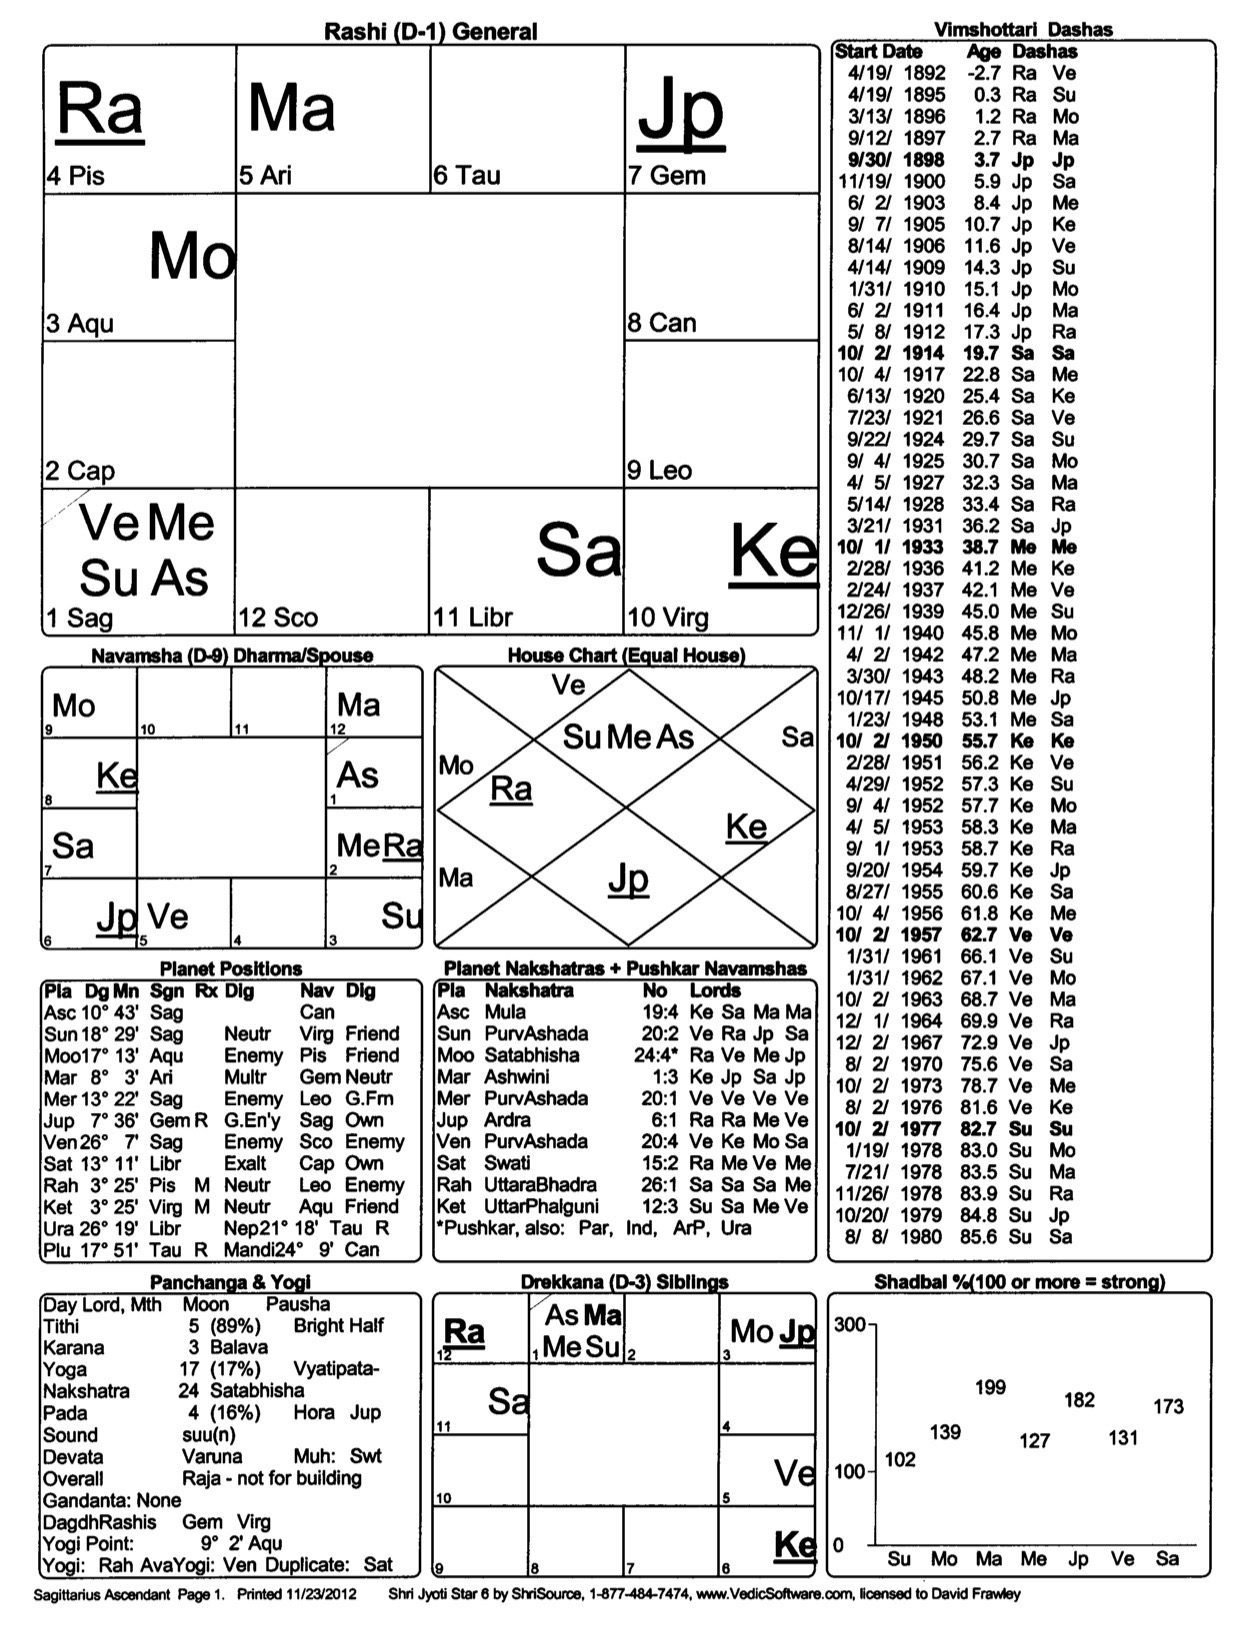
\includegraphics[width=10cm]{pics/Sagittarius-Ascendant.jpg}
\caption{}
\end{figure}
 

 

\paragraph{Indications of Sample Chart}

 

This is the chart of J. Edgar Hoover, famous FBI chief. Here I have used it to show that an apparently strong Sagittarius chart need not be highly spiritual but can be rather self-righteous, speaking of course as a former anti-war protestor in the Vietnam era. However I must admit that the chart does not show a highly afflicted character or some kind of monster as he has been portrayed. Excessive zeal was probably his main mistake.

 

Jupiter, lord of the first and fourth, is retrograde in the seventh house, from which position it aspects and boosts up its own sign. In Gemini it is in mutual exchange with the seventh and tenth lord Mercury (in Sagittarius). This creates a Raja Yoga, combining the first lord with the tenth lord, a trine with an angular house.

 

Such an exchange of first and seventh houses is often good for an actor or anyone who needs to make disguises or influence partners (I am not particularly referring to Hoovers reputation as a cross dresser, I might add). Yet Venus also in the first aspecting Jupiter as the sixth and eleventh lord adds some spice, if not paranoia to the combination, which in Hoovers case was an obsession with the criminal, the enemy or the commie. The addition of the Sun, the ninth lord, to Jupiter, the first and Mercury, the tenth lord, creates a yet more powerful Raja Yoga. The Sun as ninth lord is in the Ascendant under the influence of three benefics.

 

The entire combination in the first house is aspected by Saturn, the second and third lord, from its position in the eleventh house. This imparts more severity to his character. Saturn in the eleventh is strong in an upachaya house and also exalted. It gives material gains and administrative powers that increase with life. He eventually became the master of a huge police empire that even the President could not challenge. Saturn is strengthened by Mars, which makes it yet more severe, and by the aspect of Jupiter. Mars in the fifth in its own sign is good for legal and police activities, for advice and interrogation.

 

One might think that Jupiter in the seventh aspected by Venus and the seventh lord would give marriage. The retrograde status of Jupiter weakens this. I do not see why marriage would have to be denied, but an affliction in the Navamsha could have contributed to it. The Navamsha given here has such an affliction but with such an approximation of the birth time may not be correct.

 

The Moon, the eighth lord, is in the third house, where it is aspected by Jupiter. In a sign of Saturn it increases his detachment. At the same time the Moon in the third, a house of impulse, tends to be impulsive, erratic or even martial in its characteristics.

 

The Rahu-Ketu axis extends from the fourth to the tenth house along the other Jupiter-Mercury axis. Ketu in the tenth here gives rather archaic and inflexible attitudes in his public life. Yet Ketu is not bad here because its ruler, Mercury, is involved in a powerful Raja Yoga. Certainly Hoover served as a kind of Ketu or terminator figure on the public sphere, removing criminals and those opposed to the government.

 

\paragraph{Positions From the Moon}

 

The Moon is in Aquarius as the sixth lord, the lord of enemies, giving a more contentious nature to his disposition. Curiously the Moon is in Shatabhishak, a Nakshatra of justice and retribution. The lord of the Moon sign and the twelfth from it, Saturn, is exalted in the ninth house from the Moon, giving him high ideals and a strong sense of justice. It has the aspects of Jupiter and Mars from the fifth and the third rendering it yet more powerful and active and giving it more effect upon the mind.

 

The Sun, Mercury and Venus are in the eleventh from the Moon as rulers of the fourth, fifth and seventh, with Venus as the Yoga Karaka. This gives a strong Raja Yoga from the Moon. The Aspect of Jupiter, the eleventh lord to the eleventh house, makes this combination yet more powerful and profitable. The fifth house from the Moon, the house of advise is highly aspected and mainly by benefics and is itself a sign of Mercury aspected by its own lord.

 

\paragraph{The Navamsha}

 

The birth time is too approximate to guarantee an accurate Navamsha. However in this position we can still learn a lot by doing a little trick. We take the Ascendant in the birthchart and make it the Ascendant in the Navamsha and read positions from there.

 

If we make Sagittarius into the Navamsha Ascendant, Jupiter is in its own sign and in a mutual aspect with Mars in the seventh. A strong Sun as ninth lord is in the tenth, while Mercury as tenth lord is in the ninth, a good Raja Yoga. The Moon as eighth lord is afflicted by Saturn in the fourth. In other words, we see many of his qualities mirrored in another way.

 

\subsection{Capricorn Ascendant Chart}

\paragraph{Nature of Capricorn Ascendant}
 

Capricorn is the strongest of the two Saturn ruled Ascendants. Even though Aquarius is the mulatrikona sign of Saturn its inherent strength is weakened by Saturns rulership of the twelfth house. For Capricorn, Saturn rules the first and second houses making the person hard working and enterprising. As a movable Earth sign it gives a lot of practical initiative, though often starting from a low position in life. Both the Sun and the Moon become difficult planets, along with Jupiter and Mars. Venus is strongest and Yoga Karaka, while Mercury is tainted a bit by its sixth house rulership.

 

\begin{figure}[h]
\centering
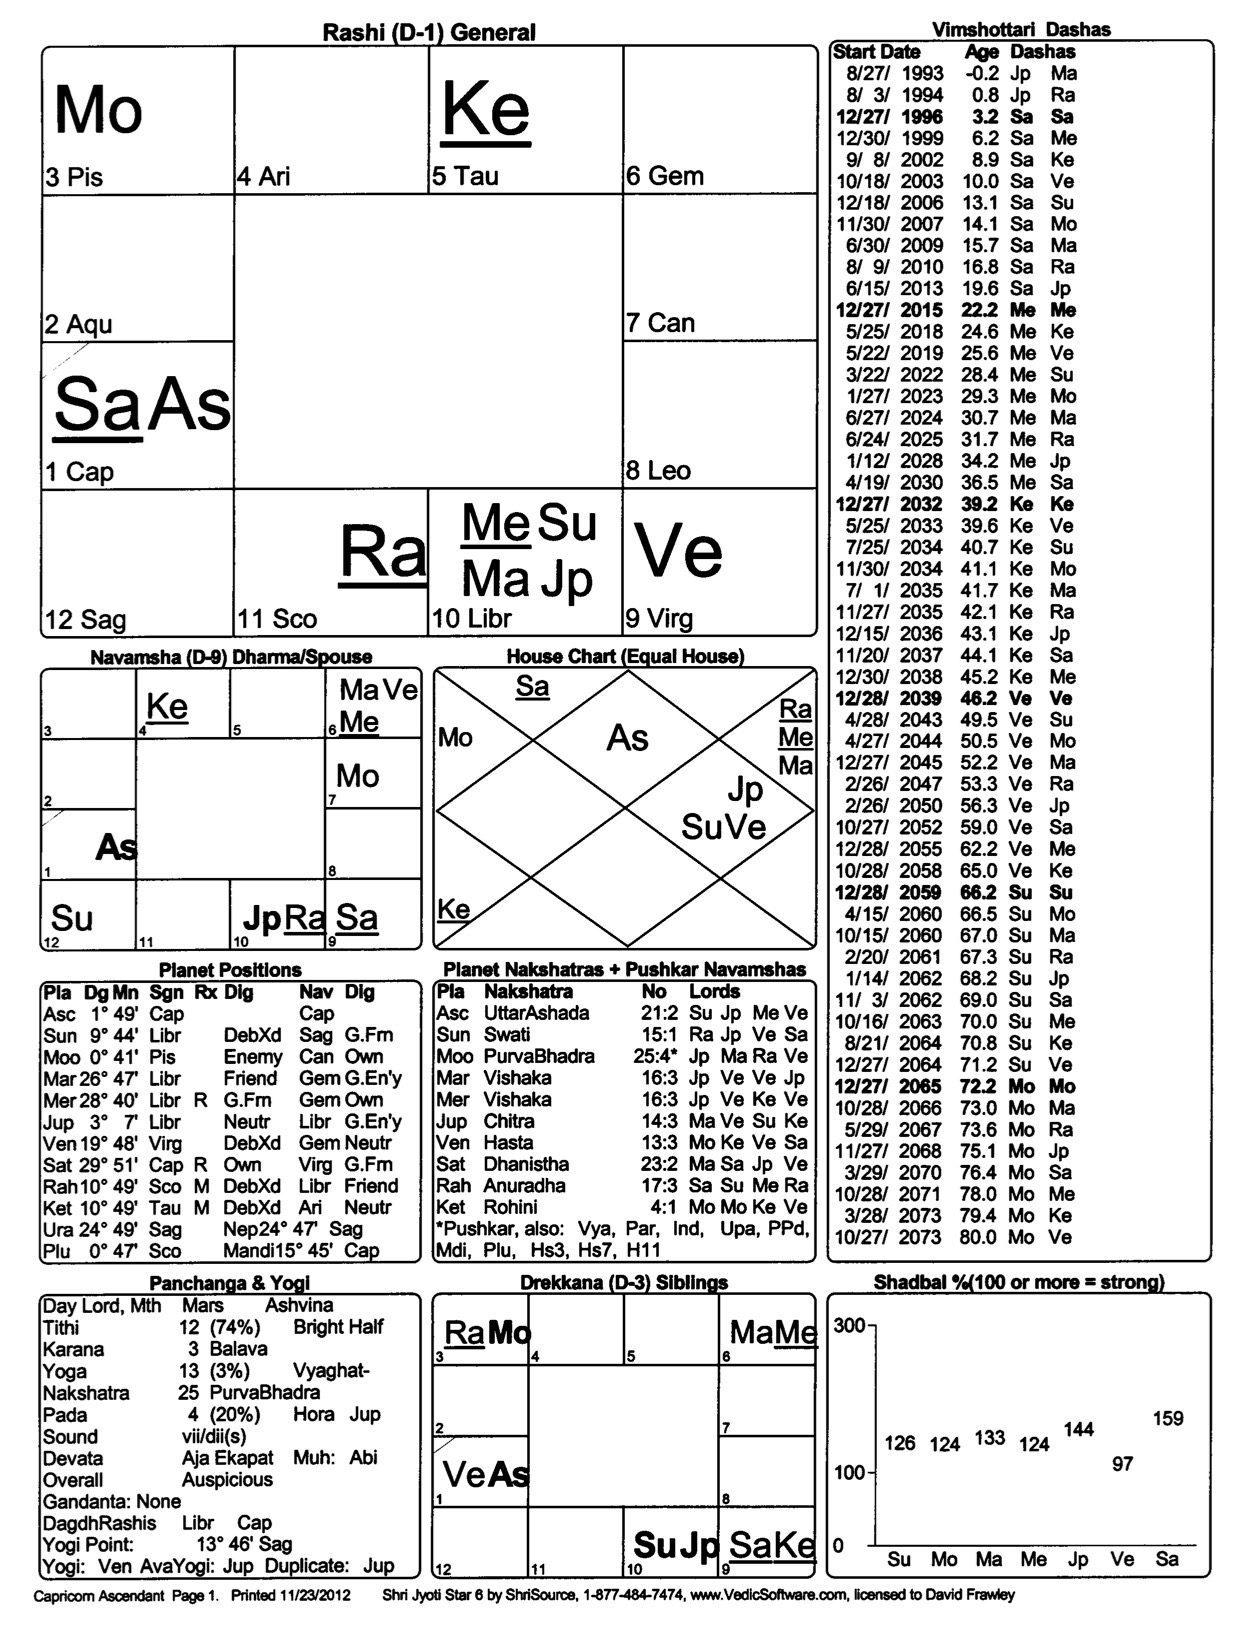
\includegraphics[width=10cm]{pics/Capricorn-Ascendant.jpg}
\caption{}
\end{figure}
 

 

\paragraph{Indications of Sample Chart}

 

This is of the child of a highly successful and proficient teacher, therapist and writer, whose wife is also a teacher. Naturally the child has not been around long enough to verify the chart by many events in the life. However as astrologers we are often asked to look at the charts of children. Generally the childs full karmic potential will not manifest until after the twelfth year, when all inhibiting past life karmas of both the child and the parent, which could harm the child, have worked themselves out. Nevertheless we can see important aspects of the childs future life from the moment of birth. The main concern in this particular chart is whether the child would follow in the footsteps of the parents and have a strong spiritual inclination or even be a great spiritual teacher.

 

Saturn, the first and second lords, is retrograde in the Lagna, which is also vargottama, strengthening it. Yet the child did have a correctable birth defect that caused the parents some worry. The retrograde nature of Saturn, the aspect of Mars on the Ascendant, and Saturns affliction of the Moon no doubt contributed to this. But the strength of the Ascendant and its lord corrected the problem.

 

Jupiter, the third and twelfth lord, is strongly placed in the tenth house, with several planets. Mars, the fourth and eleventh lord, is there. Mercury retrograde as the sixth and ninth lord is also there. The Sun as the eighth lord is there, debilitated. Generally debility of the eighth lord, which can be inimical, is more a help than a problem. Mars and the Sun benefit from being in an upachaya house and having directional strength. Jupiter suffers somewhat from being combust but gains by being vargottama.

 

Venus, the lord of the fifth and ninth, and the Yoga karaka, is in the ninth house (Gemini), exchanging signs with Mercury (Libra). This creates a powerful Raja Yoga. In this instance the debility of Venus is not very harmful. Even Mercurys retrograde aspect becomes good because this causes it to cast a greater influence back upon the sign Virgo. This powerful Raja Yoga causes the malefic planets in the tenth to be more favorable. As the Raja Yoga involves Mercury and Venus it must have an intellectual, artistic and spiritual content to it. The chart shows much mastery of the field of Earth represented by Capricorn. Such a person would be a teacher and though artistic in bent, would be serious and Saturnian as well.

 

The Moon, lord of the seventh house, is in the third, aspected by Venus and Saturn. Saturn aspects the seventh house. Venus, the significator of the wife, is debilitated. Naturally the marriage potential is limited. But the Venus-Moon aspect will at least give good relations with the opposite sex on the level of communication. Both Mars and Saturn aspects on the Moon bring in a tendency to renunciation.

 

The Rahu-Ketu axis falls upon the eleventh and fifth houses. Rahu in the eleventh is good. Ketu in the fifth is good because its lord, Venus, is so highly placed in a Raja Yoga. Ketu here in such a chart gives much spiritual knowledge and psychic insight. Hence overall the chart does show the potential of an individual who will be highly successful in life and can be an intellectual or spiritual leader.

 

\paragraph{Positions from the Moon}

 

From the Moon, the positions are not quite as favorable. The Moon is located in Pisces as the fifth lord. Jupiter, lord of the Moon sign, is located in the eighth from it. With Jupiter are the Sun, the sixth lord, Mercury, the fourth and seventh lord, and Mars, the second and ninth lord. This combination is aspected by Saturn.

 

Mercury and Venus exchange signs as rulers of the fourth and seventh with that of third and eighth creating no Raja Yoga. However, Mars and Jupiter as ninth and tenth lords do form a Raja Yoga by their combination. This suggests a strong eighth house in terms of occult and spiritual knowledge.

 

Saturn, the eleventh and twelfth lord, is located in the eleventh, a good placement for it and its mutual full aspect with Mars links the ninth and eleventh houses, giving income, gain and elevation in life. In any case the weakness of the Moon sign is compensated to a great extent by the strength of the birthchart.

 

\paragraph{Navamsha}

 

The Navamsha is vargottama, having the same sign as the birthchart, with the Moon and Jupiter in angles. Otherwise it is somewhat weak with Mercury and Venus in the sixth aspected located with malefic Mars and aspected by the Sun and Saturn. This suggests that health problems may come out again later on in life. The Navamsha does not have quite the power to support the energy and manifest all the potentials of the birthchart. Mercury and Venus constitute a Raja Yoga, but in the sixth house they may push the native to overwork or exhaustion. On the positive side they give a great capacity for service.

 

\subsection{Aquarius Ascendant Chart}
 

\paragraph{Nature of Aquarius Ascendant}

 

Aquarius is another Ascendant that is often not strong with its lord, malefic Saturn, also ruling the twelfth house. Venus is the great Yoga Karaka planet. Mercury, though generally good, suffers more than for Capricorn, because its mulatrikona house is the malefic eighth house. The Sun does not gain much through ruling an angle because it is also a maraka. The Moon is the malefic sixth lord. Jupiter, though good for business, is not auspicious and has maraka powers. Mars, though generally bad, has some benefit by ruling the tenth.

 

 \begin{figure}[h]
\centering
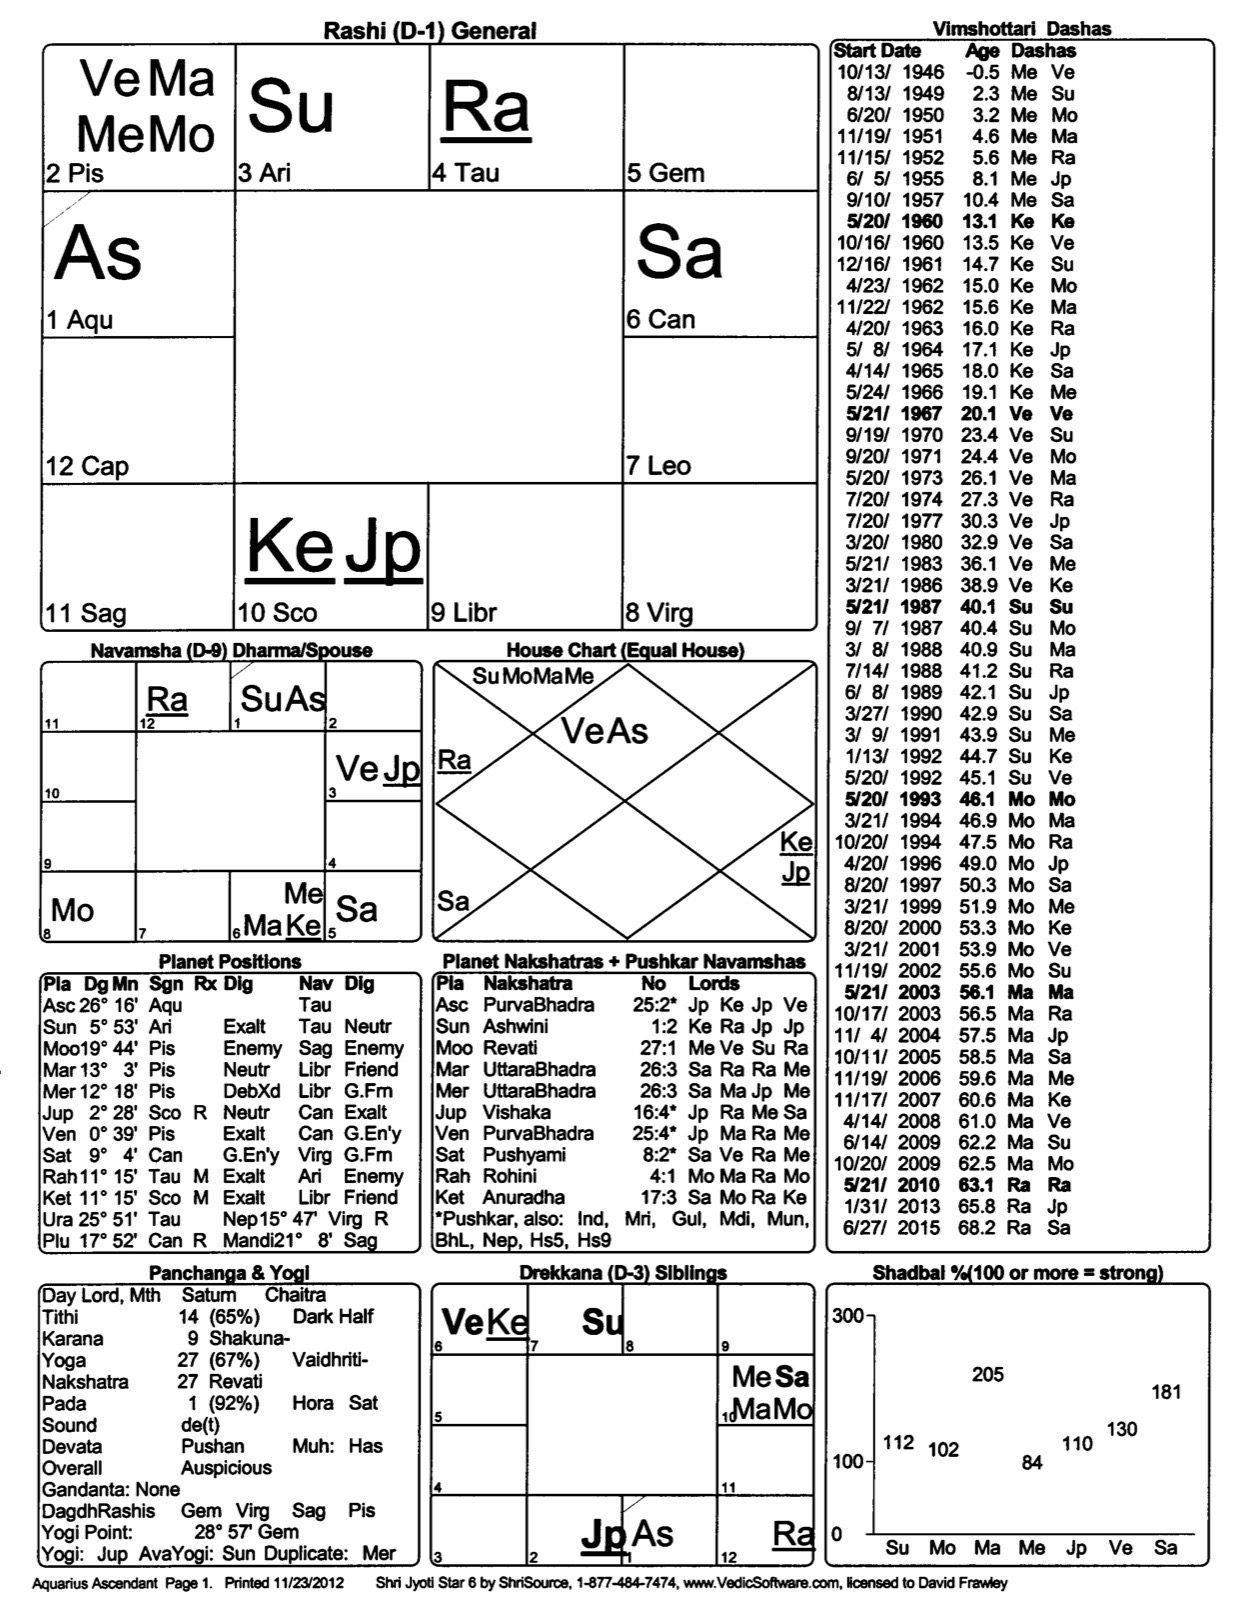
\includegraphics[width=10cm]{pics/Aquarius-Ascendant.jpg}
\caption{}
\end{figure}
 



\paragraph{Indications of Sample Chart}

 

The individual of the chart in question is a highly spiritual and artistic person who has retired from the world to live in an ashram, where he handles its library and edits an important spiritual journal. He is also talented in terms of music and chanting. He came from a highly educated and spiritual family in India.

 

The first and twelfth lord Saturn is located in the sixth house, an upachaya house. According to the rule that malefics do well in the sixth house this position, if not afflicted is quite good. It has the aspect of Jupiter, which does not harm it. The individual has a lot of curiosity and motivation in life.

 

The second and eleventh lord Jupiter is located in the tenth house and also aspects the tenth lord Mars. Jupiter and Mars exchange signs as the tenth and eleventh lords. The individual has some degree of public recognition and no material problems owing to coming from a very well educated and affluent family. Jupiter retrograde with naturally retrograde Ketu makes inclines the native further toward renunciation.

 

Mars, lord of the third and tenth, is located in the second house. As one of four planets this causes a Sannyasa Yoga or combination for renunciation. Mercury, present as the fifth and eighth lord, and Venus as the Yoga Karaka ruling the fourth and ninth, give a Raja Yoga combination. The Moon contributes to this. His writing and speaking ability no doubt get enhanced by this. Mars aspects the fifth house, Gemini, and the fifth lord, Mercury, denying children.

 

The Sun, the seventh lord, is exalted in the third. There are, however, no aspects to the seventh house. The native had a short marriage with a woman of a different community but this was not successful.

 

The natives father is highly educated and an important religious leader, running a major organization. Not only is the Sun exalted and aspecting the ninth house, the ninth lord itself is exalted, combining with the ninth and tenth lords (Mercury and the Moon) from Libra, the Ascendant for the father.

 

The Rahu-Ketu axis falls on the fourth and tenth houses. This strengthens his tendency to renunciation, particularly since Mars, the lord of Ketu, is in a Sannyasa Yoga in the second house.

 

\paragraph{Positions from the Moon}

 

Naturally with so many planets with the Moon, one should read this chart from the Moon sign as well. The Moon is the fifth lord from the Moon sign. It combines with Mars, the ninth lord from the Moon sign, and Mercury, the fourth lord, giving a Raja Yoga. Venus conjoins with it for a weak Malavya Yoga or Maha Purusha Yoga of Venus. Jupiter aspects this combination from the ninth house as the tenth and first house lord boosting it up further. Jupiter and Mars exchange signs as ninth and tenth lords. Such a Raja Yoga is colored by the Sannyasa Yoga and gives the person some position in a spiritual organization.

 

The seventh from the Moon, Virgo, and its lord Mercury a well as Venus, the karaka for marriage, are afflicted by Mars and Saturn, further removing the native from the affairs of that house. Saturn is located in the fifth from the Moon further denying the possibility of children.

 

\paragraph{The Navamsha}

 

The Navamsha confirms the afflictions of the seventh house, with the seventh house of the Navamsha aspected by the Sun, Saturn and Jupiter, while the seventh lord goes into the sixth house. The fifth house contains Saturn and Ketu, again denying children, and the fifth lord is in the difficult sixth house along with malefic Mars. Saturn as the ninth lord in the fifth house, however, does give a deep intelligence.

The Moon and Jupiter exchange houses as the third and eighth giving psychic and spiritual insight to the chart.

 

\paragraph{Additional Notes}

 

Overall the chart does indicate how a Sannyasa Yoga of the four planet combination works. What appears to be a highly emotional combination with Mars and Venus conjoined to the Moon and Mercury in watery and mutable Pisces ends up giving the person power of renunciation and devotional peace.

 

\subsection{Pisces Ascendant Chart}
 

\paragraph{Nature of Pisces Ascendant}

 

Pisces is not usually a strong Ascendant being watery and dual in qualities, and the twelfth sign. It is stronger than Virgo, its opposite, but has many of the same weaknesses. It is often an overly emotional sign and this can lead to health difficulties as well.

 

The Sun, though a natural friend of Jupiter, suffers by ruling the sixth house. Mars is the best planet, ruling the ninth, but is still a maraka, ruling the second. Mercury becomes weak as the lord of two angles. Saturn remains the worst planet as the eleventh and twelfth lord, and Venus also causes many problems ruling the third and eighth.

 

\begin{figure}[h]
\centering
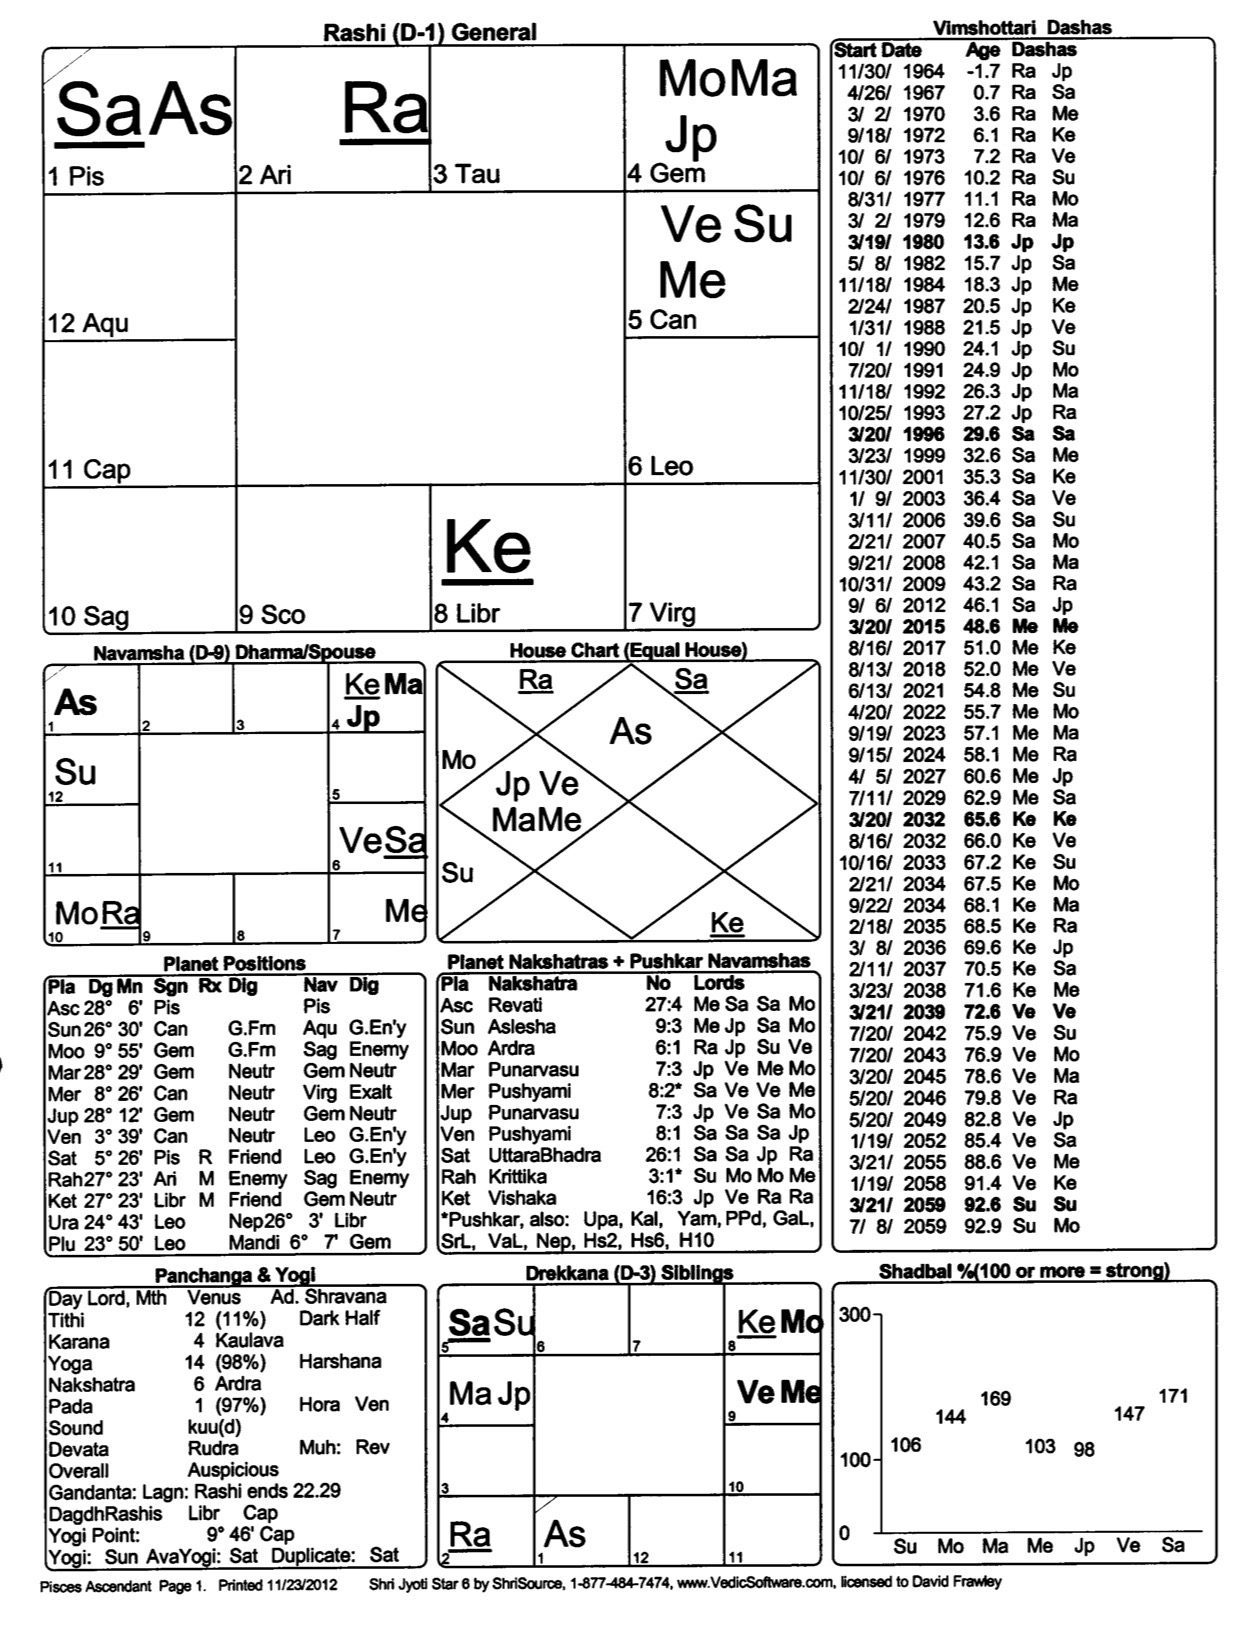
\includegraphics[width=10cm]{pics/Pisces-Ascendant.jpg}
\caption{}
\end{figure}
 

 

\paragraph{Indications of Sample Chart}

 

The following chart is of a natural healer and therapist, who does both counseling and bodywork and helps run a retreat and rejuvenation center. He is a remarkably cheerful and communicative person with much physical and emotional energy. Yet he is also humble and prefers to stay behind the scenes, helping others rather than promoting himself. This is the chart of a rare breed, a man who is emotional, sensitive, considerate and modest, a natural healer devoid of egoism.

 

Jupiter, lord of the first and tenth houses, is located in the fourth house, a place of the heart and a Moksha house. Mars, lord of the second and ninth, is also located in the fourth house. The Moon, lord of the fifth house, is similarly located in the fourth. The Moon and Mercury exchange houses as rulers of the fourth and fifth. All these are friendly planets and in a house of the emotional nature. This gives the person a happy, creative and expressive emotional nature. They also create a good Raja Yoga, combining the ninth, tenth, fourth and fifth house rulers. The Moon, Jupiter and Mars boost up the tenth house by their aspects.

 

Venus, lord of the third and eighth, is located in the fifth house. Mercury, lord of the fourth and seventh, is there as well, along with the Sun, lord of the sixth. This is a good combination for strengthening the fifth house and its spiritual and intellectual potentials. Mercury, the seventh lord, with Venus in the fifth house also give marital happiness. However Saturns aspect to the seventh house makes the wife somewhat older in age.

 

The Moon and Mercury exchange signs (Gemini and Cancer) as fourth and fifth house lords. Such good fourth and fifth houses show a harmony of emotion (fourth house) and intellect (fifth house). We have already mentioned this as a Raja Yoga.

 

However there is a limiting factor to this combination. Saturn, lord of the eleventh and twelfth, is located retrograde in the Ascendant. This is a difficult combination and creates obstacles in life, particularly in early childhood. It causes the native to underestimate his own abilities so that the potentials of the chart are not always fulfilled. Its aspect on the tenth house can be quite limiting. However, on the positive side Saturn here makes the native humble and inclines him toward Moksha, as its retrograde motion extends its influence back to the twelfth house.

 

The Rahu-Ketu axis extends from the second to the eighth house, which is also complicating, and can confuse self-expression (second house). The other benefic planets are held in check with Saturn and Rahu on one side and Ketu on the other. Whenever all the planets are hemmed in between malefics, even though the houses are not adjacent, a constricting effect or limiting effect on the life is evident. Similarly if benefics are in such a position a creative and expansive energy comes out.

 

\paragraph{Positions from the Moon}

 

The Moon is in Gemini as the second lord, along with Jupiter as the tenth lord and Mars as the eleventh lord, a strong position for gains in career and self-expression. However, the Moon, Mars and Jupiter are not good planets for Gemini and can make the native overextend himself. Saturn also goes into the tenth from the Moon as the ninth lord. This elevates the native but can bring him down at times as well.

 

The exchange between the Moon and Mercury is between the first and second lords giving good and harmonious powers of expression. The Sun, Mercury and Venus in the second as the first, third, fourth and fifth lords, give good expression and artistic abilities. Rahu-Ketu in the eleventh and fifth from the Moon are generally good and help deepen the mind.

 

\paragraph{Navamsha}

 

The Navamsha is also Pisces making it vargottama and imparting further strength to the birthchart. The Jupiter-Mars conjunction in the fourth is a Raja Yoga, combining the ninth and tenth lords. The Moon as fifth lord contributes to this, but the Rahu-Ketu axis weakens it and can cause confusion.

 

Mercury gains strength by being exalted in an angle in the seventh house, but is also afflicted by Mars. Venus and Saturn are weak in the sixth in Leo, aspected by the Sun. The Sun is weak in the twelfth house, though aspected by Jupiter it is highly spiritualized. The Navamsha, like the Lagna, shows strength to the tenth house that can be blocked.

 

\paragraph{Additional Notes}

 

The native underwent his Jupiter Dasha from March 1980 to March 1996. While there was much inner growth, his outer work, though developing, has not quite taken off. In his Saturn Dasha the public work also proved difficult, with personal set backs, and eventual withdrawal to a small practice.

